% **************************************************
% Document Class Definition
% **************************************************
\documentclass[%
    paper=A4,               % paper size --> A4 is default in Germany
    twoside=true,           % onesite or twoside printing
    openright,              % doublepage cleaning ends up right side
    parskip=half,           % spacing value / method for paragraphs
    chapterprefix=true,     % prefix for chapter marks
    11pt,                   % font size
    headings=normal,        % size of headings
    bibliography=totoc,     % include bib in toc
    listof=totoc,           % include listof entries in toc
    titlepage=on,           % own page for each title page
    captions=tableabove,    % display table captions above the float env
    chapterprefix=false,    % do not display a prefix for chapters
    appendixprefix=false,    % but display a prefix for appendix chapter
    draft=false,            % value for draft version
]{scrreprt}%


% **************************************************
% Setup YOUR thesis document in this file !
% **************************************************
% !TEX root = my-thesis.tex


% **************************************************
% Files' Character Encoding
% **************************************************
\PassOptionsToPackage{utf8}{inputenc}
\usepackage{inputenc}


% **************************************************
% Information and Commands for Reuse
% **************************************************
\newcommand{\thesisTitle}{Breaking the Shuffling Countermeasure in Lattice-Based Signature Schemes}
\newcommand{\thesisName}{Alexis Bagia}
%\newcommand{\thesisSubject}{Documentation}
\newcommand{\thesisSubject}{Bachelor's Thesis}
\newcommand{\thesisDate}{29.07.2022}
\newcommand{\thesisVersion}{Final}

\newcommand{\thesisFirstReviewer}{Prof. Dr. Jean-Pierre Seifert}
\newcommand{\thesisFirstReviewerUniversity}{\protect{Technische Universität Berlin}}
\newcommand{\thesisFirstReviewerDepartment}{Professur Security in Telecommunications}

\newcommand{\thesisSecondReviewer}{Prof. Dr. Thorsten Koch}
\newcommand{\thesisSecondReviewerUniversity}{\protect{Technische Universität Berlin}}
\newcommand{\thesisSecondReviewerDepartment}{Fachgebiet Software und Algorithmen für die\\diskrete Optimierung}

\newcommand{\thesisFirstSupervisor}{M.Sc. Vincent Quentin Ulitzsch}
%\newcommand{\thesisSecondSupervisor}{John Smith}

\newcommand{\thesisUniversity}{\protect{Technische Universität Berlin}}
\newcommand{\thesisUniversityDepartment}{Professur Security in Telecommunications}
\newcommand{\thesisUniversityInstitute}{Institut für Softwaretechnik und Theoretische Informatik}
%\newcommand{\thesisUniversityGroup}{Clean Thesis Group (CTG)}
\newcommand{\thesisUniversityGroup}{}
\newcommand{\thesisUniversityCity}{Berlin}
\newcommand{\thesisUniversityStreetAddress}{Ernst-Reuter-Platz 7}
\newcommand{\thesisUniversityPostalCode}{10587}


% **************************************************
% Debug LaTeX Information
% **************************************************
%\listfiles


% **************************************************
% Load and Configure Packages
% **************************************************
\usepackage[german,english]{babel} % babel system, adjust the language of the content
\PassOptionsToPackage{% setup clean thesis style
    figuresep=colon,%
    hangfigurecaption=false,%
    hangsection=true,%
    hangsubsection=true,%
    sansserif=false,%
    configurelistings=true,%
    colorize=full,%
    colortheme=bluemagenta,%
    configurebiblatex=true,%
    bibsys=biber,%
    bibfile=bib-refs,%
    bibstyle=alphabetic,%
    bibsorting=nty,%
}{cleanthesis}
\usepackage{cleanthesis}

\hypersetup{% setup the hyperref-package options
    pdftitle={\thesisTitle},    %   - title (PDF meta)
    pdfsubject={\thesisSubject},%   - subject (PDF meta)
    pdfauthor={\thesisName},    %   - author (PDF meta)
    plainpages=false,           %   -
    colorlinks=false,           %   - colorize links?
    pdfborder={0 0 0},          %   -
    breaklinks=true,            %   - allow line break inside links
    bookmarksnumbered=true,     %
    bookmarksopen=true          %
}

% **************************************************
% Other Packages
% **************************************************
\usepackage[colorinlistoftodos,prependcaption,textsize=tiny,disable]{todonotes}
\usepackage{dirtytalk}
\usepackage{amsthm}
\usepackage{amsmath}
\usepackage{dsfont}
\usepackage{bm}
\usepackage{minted}
\usepackage{subcaption}
\usepackage[linesnumbered]{algorithm2e}

\usepackage{scrhack}


\DeclareUnicodeCharacter{03C3}{\sigma}
\DeclareUnicodeCharacter{03C4}{\tau}
\DeclareUnicodeCharacter{03B4}{\delta}
\DeclareUnicodeCharacter{03BA}{\kappa}
\DeclareUnicodeCharacter{039B}{\Lambda}
\DeclareUnicodeCharacter{03BC}{\mu}
\DeclareUnicodeCharacter{03B2}{\beta}
\DeclareUnicodeCharacter{03B6}{\zeta}
\DeclareUnicodeCharacter{03B3}{\gamma}

\newtheorem{definition}{Definition}
\newcommand\norm[1]{\lVert#1\rVert}



% **************************************************
% Document CONTENT
% **************************************************
\begin{document}

% uncomment the following command to fill up pages with
% whitespace instead of aligning the first and last lines
% of a page (see \raggedbottom vs. \flushbottom)
%\raggedbottom

% --------------------------
% rename document parts
% --------------------------

% > set short label names for floating environments figure and table
%\renewcaptionname{ngerman}{\figurename}{Abb.}
%\renewcaptionname{ngerman}{\tablename}{Tab.}
\renewcaptionname{english}{\figurename}{Fig.}
\renewcaptionname{english}{\tablename}{Tab.}

% > rename the title of the LOL, i.e. list of listings (default is "Listings")
\renewcommand*{\lstlistlistingname}{List of Listings}

% --------------------------
% Front matter
% --------------------------
\pagenumbering{roman}			% roman page numbing (invisible for empty page style)
\pagestyle{empty}				% no header or footers
% !TEX root = ../my-thesis.tex
%
% ------------------------------------  --> cover title page
\begin{titlepage}
	\pdfbookmark[0]{Cover}{Cover}
	\flushright
	\hfill
	\vfill
	{\LARGE\thesisTitle \par}
	\rule[5pt]{\textwidth}{.4pt} \par
	{\Large\thesisName}
	\vfill
	\textit{\large\thesisDate} \\
	Version: \thesisVersion
\end{titlepage}


% ------------------------------------  --> main title page
\begin{titlepage}
	\pdfbookmark[0]{Titlepage}{Titlepage}
	\tgherosfont
	\centering

	{\Large \thesisUniversity} \\[4mm]
	
\includegraphics[width=4cm]{gfx/Clean-Thesis-Logo} \\[2mm]
	\textsf{\thesisUniversityDepartment} \\
	\textsf{\thesisUniversityInstitute} \\
	\textsf{\thesisUniversityGroup} \\

	\vfill
	{\large \thesisSubject} \\[5mm]
	{\LARGE \color{ctcolortitle}\textbf{\thesisTitle} \\[10mm]}
	{\Large \thesisName} \\

	\vfill
	\begin{minipage}[t]{.27\textwidth}
		\raggedleft
		\textit{1. Reviewer}
	\end{minipage}
	\hspace*{15pt}
	\begin{minipage}[t]{.65\textwidth}
		{\Large \thesisFirstReviewer} \\
	  	{\small \thesisFirstReviewerDepartment} \\[-1mm]
		{\small \thesisFirstReviewerUniversity}
	\end{minipage} \\[5mm]
	\begin{minipage}[t]{.27\textwidth}
		\raggedleft
		\textit{2. Reviewer}
	\end{minipage}
	\hspace*{15pt}
	\begin{minipage}[t]{.65\textwidth}
		{\Large \thesisSecondReviewer} \\
	  	{\small \thesisSecondReviewerDepartment} \\[-1mm]
		{\small \thesisSecondReviewerUniversity}
	\end{minipage} \\[10mm]
	\begin{minipage}[t]{.27\textwidth}
		\raggedleft
		\textit{Supervisor}
	\end{minipage}
	\hspace*{15pt}
	\begin{minipage}[t]{.65\textwidth}
		\thesisFirstSupervisor
	\end{minipage} \\[10mm]

	\thesisDate \\

\end{titlepage}


% ------------------------------------  --> lower title back for single page layout
\hfill
\vfill
{
	\small
	\textbf{\thesisName} \\
	\textit{\thesisTitle} \\
	\thesisSubject, \thesisDate \\
	Reviewers: \thesisFirstReviewer\ and \thesisSecondReviewer \\
	Supervisor: \thesisFirstSupervisor \\[1.5em]
	\textbf{\thesisUniversity} \\
	\textit{\thesisUniversityGroup} \\
	\thesisUniversityInstitute \\
	\thesisUniversityDepartment \\
	\thesisUniversityStreetAddress \\
	\thesisUniversityPostalCode~\thesisUniversityCity
}
		% INCLUDE: all titlepages
\cleardoublepage


\cleardoublepage
% !TEX root = ../my-thesis.tex
%
%************************************************
% Declaration
%************************************************
%\pdfbookmark[0]{Affidavit }{Affidavit}
\addchap[Affidavit / Eidesstaatliche Erklärung]{Affidavit}
\label{sec:affidavit}
\thispagestyle{empty}

I hereby declare that the thesis submitted is my own, unaided work, completed without any unpermitted external help. Only the sources and resources listed were used.

\bigskip

\noindent\textit{\thesisUniversityCity, \thesisDate}

\smallskip

\begin{flushright}
	\begin{minipage}{5cm}
		\rule{\textwidth}{1pt}
		\centering\thesisName
	\end{minipage}
\end{flushright}

\bigskip\bigskip\bigskip


%\pdfbookmark[0]{Eidesstaatliche Erklärung}{Eidesstaatliche Erklärung}
{\usekomafont{chapter}Eidesstaatliche Erklärung}
\bigskip\bigskip
\label{sec:eidesstaatliche-erklärung}
\thispagestyle{empty}

Hiermit erkläre ich, dass ich die vorliegende Arbeit selbstständig und eigenhändig sowie ohne unerlaubte fremde Hilfe und ausschließlich unter Verwendung der aufgeführten Quellen und Hilfsmittel angefertigt habe.


\noindent\textit{\thesisUniversityCity, \thesisDate}

\smallskip

\begin{flushright}
	\begin{minipage}{5cm}
		\rule{\textwidth}{1pt}
		\centering\thesisName
	\end{minipage}
\end{flushright}
\selectlanguage{english}
%*****************************************
%*****************************************



\pagestyle{plain}				% display just page numbers
% !TEX root = ../my-thesis.tex
%
\pdfbookmark[0]{Abstract / Zusammenfassung}{Abstract / Zusammenfassung}
\addchap*{Abstract}
\label{sec:abstract}

The current asymmetric cryptographic primitives which we use in our daily life are based on the hardness of the factoring and (elliptic curve) discrete logarithm problem. 
Quantum computers may in the near future become powerful enough to solve these problems and break all of our currently used asymmetric cryptographic primitives.
Because of this growing threat the the National Institute of Standards and Technology (NIST) called for proposals of post-quantum secure signature schemes and key encapsulation mechanism (KEM) already back in 2016. This resulted in extensive research on the proposed signatures schemes and KEMs, which provides reasonable assurance that they are very secure in theory.
In practice all algorithms are run on real hardware like microcontrollers and smart cards which are susceptible to physical attacks such as fault attacks. Research on possible fault attacks showed various critical parts of signature algorithms which need to be protected. One particular part in Fiat-Shamir based signature schemes is the sampling of the so-called masking polynomial, which is used to blind the linear linear relationship between the secret key and a publicly known value.
If the sampling of the coefficients of this polynomial is aborted, due to fault, some of the polynomial coefficients will be uninitialized. This will cause information about the secret polynomial to leak which can be used to recover the secret polynomial.
Different countermeasures have been proposed to prevent this attack. One among them is the shuffling countermeasure. The idea behind this countermeasure is to shuffle the order of the coefficients after they have been sampled.

Our results show that this countermeasure is not as effective as believed. Despite this shuffling countermeasure implemented we were still able to recover the secret key.
Our attack is based on Integer Linear Programs (ILPs) to recover the secret polynomial.
We show the effectiveness of our attack by extensive simulations for the signature schemes Dilithium, qTESLA as well as BLISS.
Our results highlights that the shuffling countermeasure alone is not sufficient to prevent fault attacks on the masking polynomial. Additional countermeasure are needed to properly secure upcoming microcontrollers and smart cards running post-quantum secure signature schemes against sophisticated attackers.


%\vspace*{18mm}
\pagebreak
\selectlanguage{german}
{\usekomafont{chapter}Zusammenfassung}
\label{sec:abstract-diff}
\\\phantom{{\usekomafont{chapter}Zusammenfassung}}

Die derzeitigen asymmetrischen kryptographischen Primitive, die wir in unserem täglichen Leben verwenden, basieren auf der Schwere des Faktorisierungsproblems und des diskreten Logarithmus (auf elliptischen Kurven). 
Quantencomputer könnten in naher Zukunft leistungsstark genug sein, um diese Probleme zu lösen und somit alle derzeit verwendeten asymmetrischen kryptografischen Primitive zu brechen.
Aufgrund dieser wachsenden Gefahr hat das National Institute of Standards and Technology (NIST) bereits im Jahr 2016 zur Einreichung von Vorschlägen für post-quantum-sichere Signaturverfahren und Schlüsselkapselungsmechanismen (KEM) aufgerufen.  Daraufhin wurden die vorgeschlagenen Signaturverfahren und KEMs ausgiebig erforscht und in der Theorie als sehr sicher eingestuft.
In der Praxis werden alle Algorithmen auf echter Hardware wie Mikrocontrollern und Chipkarten ausgeführt, die anfällig für physische Angriffe wie Fehlerangriffe sind. Die Forschung zu möglichen Fehlerangriffen zeigte auf, dass verschiedene kritische Bereiche von Signaturalgorithmen geschützt werden müssen.
%Ein besonderer Teil ist die Generierung des Maskierungspolynoms.
Ein besonderer Teil der auf Fiat-Shamir mit Abbruch basierenden Signaturverfahren ist die Generierung des so genannten Maskierungspolynoms, das verwendet wird, um die lineare Beziehung zwischen dem geheimen Schlüssel und einem öffentlich bekannten Wert zu verbergen.
Wenn die Generierung der Koeffizienten dieses Polynoms aufgrund eines Fehlers abgebrochen wird, werden einige der Polynomkoeffizienten nicht initialisiert. Dies führt zum Preisgabe von Informationen über das geheime Polynom, welche zur vollständigen Wiederherstellung des geheimen Polynoms verwendet werden können.
Es wurden verschiedene Gegenmaßnahmen vorgeschlagen, um diesen Angriff zu verhindern. Eine davon ist die Mischen-Gegenmaßnahme. Die Idee hinter dieser Gegenmaßnahme besteht darin, die Reihenfolge der Koeffizienten nach der Abtastung zu mischen.

Unsere Ergebnisse zeigen, dass diese Gegenmaßnahme nicht so effektiv ist wie angenommen. Trotz dieser Gegenmaßnahme war es uns möglich, den geheimen Schlüssel wiederherzustellen.
Unser Angriff basiert auf ganzzahliger linearen Optimieung (Integer Linear Program, ILP), um das geheime Polynom wiederherzustellen.
Wir zeigen die Wirksamkeit unseres Angriffs durch umfangreiche Simulationen für die Signaturverfahren Dilithium, qTESLA und BLISS.
Unsere Resultate zeigen, dass die Mischen-Gegenmaßnahme allein nicht ausreicht, um Fehlerangriffe auf das Maskierungspolynom zu verhindern. Es sind zusätzliche Gegenmaßnahmen erforderlich, um zukünftige Mikrocontroller und Chipkarten, auf denen post-quantum-sichere Signaturverfahren eingesetzt werden, gegen raffinierte Angreifer zu schützen.

\selectlanguage{english}
		% INCLUDE: the abstracts (english and german)
\cleardoublepage




%
%% !TEX root = ../my-thesis.tex
%
\pdfbookmark[0]{Acknowledgement}{Acknowledgement}
\addchap*{Acknowledgement}
\label{sec:acknowledgement}

\Blindtext[2][2]
 % INCLUDE: acknowledgement
%\cleardoublepage
%
\currentpdfbookmark{\contentsname}{toc}
\setcounter{tocdepth}{2}		% define depth of toc
\tableofcontents				% display table of contents
\cleardoublepage

% --------------------------
% Body matter
% --------------------------
\pagenumbering{arabic}			% arabic page numbering
\setcounter{page}{1}			% set page counter
\pagestyle{scrheadings}			% header and footer style

%% Uncomment the following lines using the \part command
%% to add part sections
%\part{Example Part}
\listoftodos
% !TEX root = ../my-thesis.tex
%

\chapter{Introduction}
The potential advent of large-scale quantum computers threatens to undermine the security of currently used public-key cryptography. Virtually all public-key cryptography that is used right now is based on either the hardness of factoring or discrete logarithm problems. Using Shor's algorithm \cite{shor}, large enough general-purpose quantum computers will be able to break these problems, rendering the respective public-key cryptography insecure.
Because of this the National Institute of Standard and Technology (NIST), in an effort to standardize post-quantum  cryptography, called for proposals for post-quantum secure cryptographic schemes \cite{nistcall}, i.e., schemes that withstand quantum adversaries. The call encompasses signature, encryption and key encapsulations algorithms that can be used in a potential quantum computer era.

The standardization process is currently in the fourth round, with various proposed candidates being eliminated because they were found to be insecure or impractical and some candidates already selected for standardization \cite{niststatus}. The remaining and selected candidates have thus been subject to thorough theoretical analysis.  However, the corresponding implementations require scrutiny on the implementation security, since existing cryptoanalytic efforts focused mainly on the schemes' designs. The foreseeable execution platforms for post-quantum cryptography algorithms include microcontrollers and smart cards, to, e.g., sign banking transactions. Smart cards and microcontrollers are subject to physical attacks, such as fault injection attacks. Especially for public-key cryptography like signature schemes, fault attacks can break the security of a device running a poorly implemented algorithm easily. 
Fault attacks cause the device signing a message to perform a miscalculation and therefore leak secret information. Past research demonstrated fault attacks that revealed  the entire secret with only single or a few faulty signatures \cite{faultseifert}. Designing efficient and effective countermeasures against fault-injection attacks is non-trivial, given the powerful attack primitive that they need to defend against. 

In this thesis, we will investigate the effectiveness of one specific fault-injection countermeasure against so-called loop-abort fault attacks.
%We will focus on lattice-based signature schemes, because the by the NIST to be standardized and recommended signature scheme for PQC is Dilithium \cite{niststatus}, a lattice based signature scheme.
We will focus in lattice based signature schemes because two out of the three signature schemes the NIST will standardize are based in lattices. Additionally the currently recommended PQC signature scheme is Dilithium, a lattice based signature scheme.

Prior work by Espitau et al. \cite{espitau} has shown that lattice-based signature schemes based on Fiat-Shamir with aborts (over ideal lattices) leak secret information if a masking polynomial is not properly sampled. Fault injections can cause such an improper sampling and thus can be used to reveal the secret key. To mitigate this attack, a proposed countermeasure is to randomize the order the sampling of the masking polynomial, i.e. shuffling the order of its coefficient \cite[p.~155]{espitau}. A second countermeasure was to check whether the upper few coefficients are zero and abort if too many are zero  \cite[p.~155]{espitau}. 

\section{Our Contribution}
This thesis shows that the shuffling countermeasure is not as effective as believed. We formulate Integer Linear Programs (ILPs) that can recover the secret key effectively from faulted signatures, even if the shuffling countermeasure is present. The described attack affects the implementation security of signature schemes like BLISS, qTESLA as well as the signature scheme Dilithium \cite{bliss,qtesla,dilithium}.
Dilithium is the winner of the NIST Post-Quantum-Cryptography standardization process \cite{niststatus}.  It can thus be assumed that it will be implemented a lot in the near future.
We will validate the effectiveness of our attack by extensive simulations for all the aforementioned PQC signature schemes.

Furthermore our results will show that we can even prevent the \say{checking for zero} countermeasure for Dilithium and qTESLA as we only require 1 or 2 zeroed coefficients per signature. For a single signature this can happen naturally with a high probability and thus can not be detected.

Our results will highlight the need for further research into securing the implementations of lattice-based signature schemes against fault attacks.   % INCLUDE: introduction
% !TEX root = ../my-thesis.tex
%
\chapter{Background}
This section will provide the reader with the required knowledge to understand the attack presented in this paper. First we will introduce the basic concepts of identification and signature schemes, then we will discuss the mathematical concepts of lattices and the computational problems lattice-based cryptography is based upon. Finally we will provide brief information about fault attacks in general.

\section{Identification and signature schemes}
In the public key setting signature schemes are constructions which allow to digitally sign messages. Messages can be can be anything that can be represented with zeroes and ones, e.g. PDF-files, software, videos and photos.

Just like analog signatures digital signatures have the property that they can be efficiently created, that they are valid just for a specific message, that everyone else can verify if a message-signature pair is authentic and that the signer is not able to deny a signature which is valid.

Formally Katz and Lindell \cite[p.~442]{katzlindell} describe a signature scheme as follows:

\begin{definition}[Signature Scheme]
A \textnormal{(digital) signature scheme} consists of three probabilistic polynomial-time algorithms \textnormal{(Gen, Sign, Vrfy)} such that:
\begin{enumerate}
    \item The \textnormal{key generation algorithm Gen} takes as input a security parameter $1^n$ and outputs a pair of keys (pk, sk). These are called the \textnormal{public key} and \textnormal{private key}, respectively. We assume that pk and sk each has length at least $n$. and that $n$ can be determined from pk or sk.
    
    \item The \textnormal{Sign algorithm} takes as input a private key sk and a message $m$ from some message space (that may depend on pk). It outputs a signature $\sigma$, and we write this as $\sigma \leftarrow \textnormal{Sign}_{\textit{sk}}(m)$. 
    
    \item The determininistic \textnormal{verification algorithm Vrfy} takes as input a public key pk, a message $m$, and a signature $\sigma$. It outputs a bit $b$, with $b = 1$ meaning \textnormal{valid} and $b = 0$ meaning \textnormal{invalid}. We write this as $b := \textnormal{Vrfy}_{\textit{pk}(m, \sigma)}$.
\end{enumerate}
It is required that except with negligible probability over (pk, sk) output by $\textnormal{}{Gen}(1^n)$, it holds that $\text{Vrfy}_{\textit{pk}}(m, \text{Sign}_{\textit{sk}}(m)) = 1$ for every (legal) message $m$.

If there is a function $l$ such that for every (pk, sk) output by $\text{Gen}(1^n)$ the message space is $\{0,1\}^{l(n)}$, then we say that \textnormal{(Gen, Sign, Vrfy)} is a \textnormal{signature scheme for messages of length $l(n)$}.
\end{definition}





\section{Lattices}
The general definition of a lattice is as follows:
\begin{definition}[Lattice]
A $n$-dimensional lattice $Λ$ is a discrete subgroup of $\mathds{R}^n$.
\end{definition}

Lattices are often defined by $k$ linearly independent basis vectors $b_1, \ldots, b_k \in \mathds{R}^n$.
Given these basis vectors, the corresponding lattice $Λ(b_1, \ldots, b_k)$ is defined as $Λ(b_1, \ldots, b_k) =  \{\sum_{i = 1}^k a_i b_i \vert a_i \in \mathds{Z}\}$.
In cryptography the lattices of interest are mostly discrete subgroups of $\mathds{Z}^n$ or $\mathds{Z}_q^n$ and in practice most modern lattice based cryptographic lattice primitives use so called ideal lattices. These kind of lattices were first introduced by Lyubashevsky and Micciancio \cite[p.~149]{idealdef} and they define them as follows:

\begin{definition}[Ideal Lattice]
An ideal lattice is an integer lattice $Λ(b_1, \ldots, b_k) \subseteq \mathds{Z}_n$ with $b_1, \ldots, b_k \in \mathds{Z}_q$ being the basis vectors of that lattice, such that $Λ(b_1, \ldots, b_k) = \{g \bmod f \vert g \in I\}$ for some monic polynomial $f$ of degree $n$ and ideal $I \subseteq \mathds{Z}[x]/(f)$.
\end{definition}

These ideal lattices have the great advantage that they can reduce public and private key sizes and, if proper parameters are chosen, the ring operations (multiplying polynomials) can be performed very efficiently using the number theoretic transform (NTT) \cite{ntt} speeding up the computations significantly. While the general definition of ideal lattice is hard to grasp, in this thesis we will only deal with the ideal lattice of the form $\mathds{Z}[x]/(x^n + 1)$. These kind of lattices have the additional property that they are nega-cyclic, meaning that if the vector $(a_1, a_2, \ldots, a_{n-1}, a_n)$ is in in the lattice, the rotated and negated vector $(-a_n, a_1, \ldots, a_{n-2}, a_{n-1})$ is also in the lattice \cite[p.~166]{negadesc}.


Next we introduce two basic properties of lattices which are often of great interest:

\begin{definition}[Shortest Vector]
A shortest vector of a lattice $Λ$ according to a norm $\norm{\cdot}$ is a nonzero lattice vector $v \in Λ \setminus \{0\}$ such that for all $w \in Λ \setminus \{0\}$ it holds that $\norm{v} \leq \norm{w}$.
\end{definition}

\begin{definition}[Closest Vector]
Given a $n$-dimensional lattice $Λ$ and a point $p \in \mathds{R}^n$ and a norm $\norm{\cdot}$
a closest vector to the point $p$ is a vector $v \in Λ$ such that for all $w \in Λ$ it holds that $\norm{p - v} \leq \norm{p - w}$.
\end{definition}


%\subsection{Closest Vector to a point $w \in \mathds{R}^n$}
%The closest vector to a point $w \in \mathds{R}^n$ is a vector $v \in Λ$ which is, according to a metric to a metric, closest to $v$.


\subsection{Lattice Problems}
Lattice problems are problems which are related to lattices. Such problems are used to build lattice-based cryptographic primitives.
The Closest Vector Problem (CVP) and the Shortest Vector Problem (SVP) are the fundamental problems of lattice based cryptography as they have been well studied and they appear to be resistant against quantum computers. They are defined as follows:

\begin{definition}[Shortest Vector Problem (SVP)]
Given $k$ basis vectors $b_1, \ldots, b_k \in \mathds{R}^n$ which define the lattice $Λ(b_1, \ldots, b_k)$, find a shortest vector in $Λ(b_1, \ldots, b_k)$.
\end{definition}

\begin{definition}[Closest Vector Problem (CVP)]
Given $k$ basis vectors $b_1, \ldots, b_k \in \mathds{R}^n$ which define the lattice $Λ(b_1, \ldots, b_k)$ and a point $p \in \mathds{R}^n$, find a closest vector $v \in Λ(b_1, \ldots, b_k)$ which is closest to $p$.
\end{definition}

In lattice-based cryptography new problems which are developed to build a basis for new cryptographic schemes often prove their hardness by reduction, i.e. showing that if one can solve the new problem, one can also solve CVP or SVP.

Using such reductions, the entire lattice based cryptography is based on solid foundations.

\subsubsection{Short Integer Solutions Problem}
The Short Integer Solution (SIS) problem was first introduced Ajtai in 1996 \cite{sis}.
It is defined as follows:
\begin{definition}[Short Integer Solution (SIS)]
Let $A \in \mathds{Z}_q^{m \times n}$ chosen uniformly at random. According to a norm $\norm{\cdot}$, find a vector $x \in \mathds{Z}_q^n$ such that $Ax = 0$ and $\lvert \lvert x \rvert \rvert$ is small and non-trivial.
\end{definition}

Ajtai showed in his work \cite{sis}  that that if one is able to solve the SIS problem with probability at least $\frac{1}{2}$ one can solve SVP with a probability near 1. Thus the SIS problem is at least as hard as SVP. The SIS problem is used by many latticed-based cryptographic schemes to prove their security.






\subsubsection{Ring-LWE and the Module-Ring-LWE}
The  Learning with Errors over Rings problem, also referred as search-RLWE and the generalized variant which is known as Module-LWE or Ring-Module-LWE form the foundations for many lattice based signature and key encapsulation schemes.

Here we will give a more concrete definitions than the original ones \cite{rlwe,glwe} which will be just as general enough to cover all signature schemes we will discuss here.

First we will describe the ring we will be working with:
Let $n$ be a power of two. Let $q$ be an odd prime. Let $\mathds{Z}_q$ be the ring of integers modulo $q$. Then we define the ring $\mathcal{R}_q = \mathds{Z}_q[x]/(x^n+1)$.
 
 Next both problems require some sort of error distribution $\chi$. We will either use the discrete gaussian distribution centered at zero with standard derivation $σ$ or %a uniform one, centered at zero.
 a uniform distribution over a integer range, e.g. $[-(2^{21} - 1), 2^{21} - 1] \cap \mathds{Z}$.
 
 The search variant of the Ring-LWE problem is defined as follows:
 \begin{definition}[Ring-LWE]
 For a given $s \in \mathcal{R}_q$, given pairs of the form $(a_i, b_i = a_i \cdot s + e_i) \in \mathcal{R}_q \times \mathcal{R}_q$, where $a_i \in \mathcal{R}_q$ with coefficients uniformly at random and $e_i$ chosen according to $\chi$, find $s$.
 \end{definition}
 
 The Module-Ring-LWE problem can be seen as an generalization of the Ring-LWE problem:
\begin{definition}[Module-Ring-LWE]
For a given $\bm{s} \in \mathcal{R}_q^k$, given pairs of the form $(\bm{a}_i, b_i = \langle \bm{a}_i, \bm{s} \rangle + e_i) \in \mathcal{R}_q^k \times \mathcal{R}_q^k$, where $\bm{a}_i \in \mathcal{R}_q^k$ with polynomials with coefficients uniformly at random and $e_i$ chosen according to $\chi$, find $\bm{s}$.
\end{definition}

We can see that for $k = 1$ the Module-Ring-LWE problem is the same as the Ring-LWE problem.

\section{Fiat-Shamir with aborts}
Fiat-Shamir with aborts describes a lattice based identification scheme as well as a lattice-based signature scheme, first introduced by Lyubashevsky \cite{fiatshamirabort}.   This identification scheme uses a provable collision resistant lattice-based hash function. Based on this identification scheme Lyubashevsky used the Fiat-Shamir heuristic \cite{fiatshamir} to construct a lattice-based signature scheme. The general design is used by many more recent lattice-based signature schemes such ass BLISS, Dilithium as well as qTESLA.


The Fiat-Shamir with aborts identification scheme has the general structure of a sigma-protocol: First the prover commits to a value, the commitment value, then the challenger sends a value, the so called challenge, to the prover. The prover then performs an operation using the commitment value, challenge and secret key which proves the challenger that he indeed possesses the secret key. The novelty the Fiat-Shamir with aborts scheme is that the prover may abort the identification process. In this case nothing is proven to the challenger.

The aborts allow the scheme to use smaller masking values which reduces signature size while still keeping the scheme secure.

Both, the identification scheme as well as the signature scheme, can work over the ring $\mathcal{R}_q = \mathds{Z}_q[x] / (x^n + 1)$ and require a linear collision resistant hash function $h: \mathcal{R}_q^m \mapsto \mathcal{R}_q$ from a set $\mathcal{H}$ of collision resistant hash functions.

\subsection{The identification scheme}
The private key of the prover is a vector $\bm{s} \in D_s^m$ from a secret key domain $D_s$.
The public key is the hash function $h \in H$ as well as $S = h(\bm{s})$.

The commitment value is calculated by choosing a random $\bm{y} \in D_y^m$ from a commitment domain and calculating $Y = h(\bm{y})$.
Next the challenger chooses an $c \in D_c$ from a challenge domain $D_c$. The prover then computes $\bm{z} = \bm{s}c + \bm{y}$, aborts if $\bm{z}$ is not in a good range, i.e. $\bm{z} \notin G^m$, and otherwise sends $\bm{z}$ to the challenger.

The verifier accepts if $\bm{z} \in G^m$ and $h(\bm{z}) = Sc+Y$. The scheme is correct because $h(\bm{z})= h(\bm{s} c) + h(\bm{y}) = h(\bm{s}) c + h(y) =Sc+Y$.

This identification scheme is considered secure as it is proven that if an attacker can break the scheme he can also break an approximated version of SVP.

\subsection{The signature scheme}
The signature scheme is similar to the identification scheme. It differs from the identification scheme mainly in that it additionally requires a random oracle $H$ and that the challenge $c$ is replaced by $e = c = H(h(\bm{y},\mu))$, where $μ$ is the message. Replacing the challenge with the random oracle removes the needed interaction between the two parties. In detail the signature scheme is described in Figure \ref{fig:abortsig}. The scheme is correct because $H(h(\bm{z}) - Sc, \mu) = H(h(\bm{s} c + \bm{y}) - Sc, \mu) = H(S c + Y - Sc, \mu) = H(Y, \mu)$.

\begin{figure}[h]
\centering
\fbox{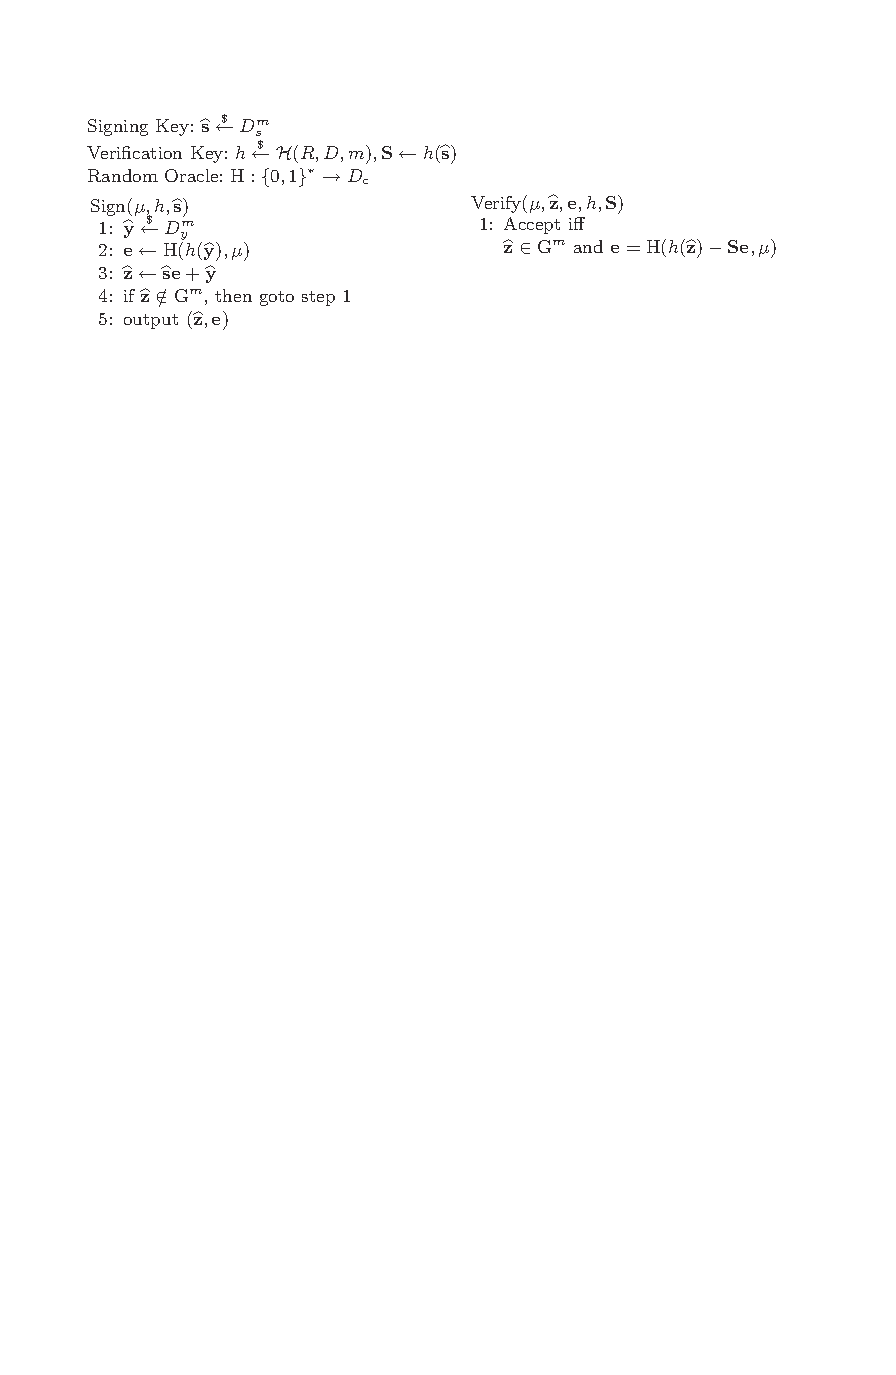
\includegraphics[width=.99\linewidth,trim=40 500 55 54,clip]{plots/loopabortsig}}
\caption{The Fiat-Shamir with aborts signature scheme. Figure copied from \cite[p.~611]{fiatshamirabort}.}
\label{fig:abortsig}
\end{figure}

\section{Lattice based signature schemes}
In this section we will briefly explain the how the signature schemes we will attack work. For each signature we will explain the key generation, the signature generation and the signature verification.
%\todo{write something here}
\subsection{Dilithium}
\label{sec:explaindilith}
Dilithium is currently the only PQC signature scheme that is both recommended and to be standardized by the NIST. \cite{niststatus} The authors proposed parameter sets for the NIST security levels 2, 3 and 5 \cite[pp.~16--17]{dilithium_spec}.

The signature works over the ring $\mathcal{R}_q = \mathds{Z}_q[x]/(x^n+1)$ where $q$ is an odd prime. Simplified works as follows:
\begin{itemize}
    \item \textbf{Key generation} First a $k \times l$ matrix $\bm{A}$ of polynomials with uniform coefficients in $\mathds{Z}_q$ is sampled as well as two secret vectors $(\bm{s}_1, \bm{s}_2) \in S_\eta^l \times S_\eta^l$. $S_\eta^k$ and $S_\eta^l$ denote the set of vectors of polynomials with coefficients with absolute value no more than $\eta$ with $k$ or $l$ entries respectively.
    Then the vector $\bm{t} = \bm{A}\bm{s}_1 + \bm{s}_2$ is calculated.
    Finally the public key is the pair $(\bm{A}, \bm{t})$ and the private key is the tuple $(\bm{A}, \bm{t}, \bm{s}_2, \bm{s}_2)$.
    
    \item \textbf{Signature generation}
    First the vector $\bm{y} \in \tilde{S}_{\gamma_1}^l$ is sampled. The only difference between $\tilde{S}_{\gamma_1}^l$ and $S_{\gamma_1}^l$ is that $\tilde{S}_{\gamma_1}^l$ does not contain any polynomial with coefficient $-\gamma_1$.
    Then the high bits of $\bm{w}_1 = \bm{A}\bm{y}$ together with the message $M$ are hashed to the ball $B_\tau$. The Ball $B_\tau$ is the set of polynomials with exactly $\tau$ coefficients being $-1$ or $1$ and the rest zero. The output of the hash function is the commitment value (commitment polynomial) $c$.
    Finally the vector $\bm{z} = \bm{y} + c \bm{s_1}$ is calculated. If $\bm{z}$ passes a tests which ensures that no information about the secret polynomials is leaked, the signature defined as the pair $\sigma = (\bm{z}, c)$ is outputted. Otherwise the process will be repeated until a generated signature passes the tests and can be outputted.
    
    \item \textbf{Verification}
    To verify a signature $\sigma$ of a message $M$ according to a public key \textit{pk} the high bits of $\bm{w}_1 = \bm{A} \bm{z} - c \bm{t}$ are calculated, we name them $\bm{w}_1'$. Then the signature is accepted iff $\norm{\bm{z}}_\infty \leq \gamma_1 - \beta$ and $c = H(M \Vert \bm{w}_1')$.
\end{itemize}
This simplified version of the Dilithium signature scheme is also depicted in Algorithm \ref{alg:dilithium}.

To see why the scheme is correct the interesting part is the second condition which is checked. The question is whether following holds:
\begin{align}
\label{dilithium_correct}
	c = H(M \Vert \bm{w}_1') = H(M \Vert \text{HighBits}(\bm{A}\bm{y}))  \overset{?}{=}  H(M \Vert \text{HighBits}(\bm{A} \bm{z} - c \bm{t}))
\end{align}
We know that
\begin{align}
	\bm{A} \bm{z} - c \bm{t} = \bm{A}\bm{y}+c\bm{A}\bm{s}_1 - c\bm{A}\bm{s}_1 - c \bm{s}_2 = \bm{A}\bm{y}- c \bm{s}_2
\end{align}
Per definition of the $c$ and $\bm{s}_2$ the coefficients of  $c \bm{s}_2$ can be at most $β$. Because $β$ is comparatively small this addition / subtraction does not affect the high bits of  $\bm{A}\bm{y}$. Thus the equation \eqref{dilithium_correct} holds and the signature scheme is correct.

The security of the scheme is based on the hardness of the Module-LWE problem as well as the SIS problem.

The actual scheme contains many improvements to decrease the memory footprint, decrease execution time and the amount of entropy required but these details are not required for understanding our fault attack nor do they affect our attack.

\begin{algorithm}
\SetKwProg{Fn}{Function}{ is}{end}


\SetKwFunction{Gen}{Gen}
\SetKwFunction{Sign}{Sign}
\SetKwFunction{Verify}{Verify}

\SetKwFunction{HighBits}{HighBits}
\SetKwFunction{LowBits}{LowBits}

\Fn{\Gen{}}{
		$\bm{A} \gets R_q^{k \times l}$\;
		$(\bm{s}_1, \bm{s}_2) \gets S_{\eta}^l \times S_{\eta}^k$\;
		$\bm{t} \gets \bm{A} \bm{s}_1 + \bm{s}_2$\;
		\Return (\ArgSty{pk} $= (\bm{A}, \bm{t})$, \ArgSty{sk} $= (\bm{A}, \bm{t}, \bm{s}_1, \bm{s}_2)$)\; 
}

\SetKwFunction{H}{H}
\Fn{\Sign{sk $= (\bm{A}, \bm{t}, \bm{s}_1, \bm{s}_2)$, M}}{
		$\bm{z} \gets \bot$\;
		\While{$\bm{z} = \bot$}{
			$\bm{y} \gets \widetilde{S}^{l}_{\gamma_1}$\;
			$\bm{w}_1 \gets$ \HighBits{$\bm{Ay}, 2 \gamma_2$}\;
			$c \in B_{\tau} \gets$ \H($M \Vert \bm{w}_1$)\;
			$\bm{z} \gets \bm{y} + c \bm{s}_1$\;
			\If{$\norm{\bm{z}}_\infty \geq \gamma_1-\beta$ or \LowBits{$\bm{A}\bm{y} - c \bm{s}_2$} $\geq γ_2 - β$}{
				$\bm{z} \gets \bot$\;
			}
		}
		\Return $σ = (\bm{z}, c)$
}

\Fn{\Verify{pk $= (\bm{A}, \bm{t})$, M, $σ = (\bm{z}, c)$}}{
	$\bm{w}_1' \gets$ \HighBits{$\bm{A}\bm{z}$, $2γ_2$}\;
	\eIf{$\norm{\bm{z}}_\infty < γ_1 - β$ and $c =$ \H{$M \Vert \bm{w}_1'$}}{
		Accept
	}{
		Reject
	}
}


\caption{Simplified Dilithium signature scheme.}
\label{alg:dilithium}
\end{algorithm}

\subsection{qTESLA}
The qTESLA signature scheme \cite{qtesla} was selected for the second round of the NIST post-quantum cryptography standardization project but was not selected for round three.
When describing the scheme we will leave out various checks which are performed during key generation, signature generation and verification and also some implementation details. The checks include the rejection sampling
but also various checks which aim to counteract fault attacks. None of these checks detect our fault attack because our attack produces perfectly valid signatures. For the reader interested in all details of this signature scheme we refer to \cite{qtesla}.

\subsubsection{Notation}
qTESLA uses the ring, $\mathcal{R}_{q} = \mathds{Z}_{q}[x] / (x^{n} + 1)$ with $n \in \{1024, 2048\}$ and $q$ an odd prime. The set $\mathcal{R}_{[B]} \subseteq \mathcal{R}_q$ is defined as $\mathcal{R}_{[B]} = \{\sum_{i=0}^{n-1}f_{i}x^{i} \in \mathcal{R} \vert f_{i} \in [-B, B]\}$ and the set $\mathds{H} \subseteq \mathcal{R}_q$ is defined as $\mathds{H} = \{\sum_{i=0}^{n-1}f_{i}x^{i} \in \mathcal{R} \vert f_{i} \in \{-1, 0, 1\}, \sum_{i=0}^{n-1}f_{i} = h\}$, $h \in {25, 40}$. The $[\cdot]_M$ operator rounds aways the last few bits of its argument, roughly speaking. $G$ and $H$ are hash functions. $H$ applies the rounding operation $[\cdot]_M$ to any polynomials from $\mathcal{R}_q$ it receives as input.

\subsubsection{Key generation}
From an initial so called \say{pre-seed}, a $κ$ bit long uniform random bitstring, multiple different seeds like $\textbf{seed}_{y}$ and  $\textbf{seed}_{a}$ are generated to be used to sample the following polynomials.
First the public key polynomials $a_{1}, \ldots, a_{k}$ are sampled uniformly from $\mathcal{R}_{q}$ using $\textbf{seed}_{a}$.
Next the secret polynomial $s \in \mathcal{R}_q$ is sampled with coefficients distributed following the discrete Gaussian distribution with standard deviation $\sigma$.
The error polynomials $e_{1}, \ldots, e_{k} \in \mathcal{R}_q$ are sampled just like $s$ was sampled previously.
The public key polynomials $t_{i}$ are then calculated as $t_{i} = a_{i} s + e_{i}$ for $i \in {1, \ldots, k}$.
Finally the value $g$ is crafted by hashing all public key polynomials $t_{i}$ using $H$.
The secret key is then the tuple $(s, e_{i}, \ldots, e_{k}, \textbf{seed}_{a},  \textbf{seed}_{y}, g)$ and the public key is $(t_{1}, \ldots, t_{k},  \textbf{seed}_{a})$.

\subsubsection{Signature generation}
When signing a message $m$, first a randomness $r$ is collected. Based on this randomness the masking polynomial $y$ is sampled uniformly from $\mathcal{R}[B]$.
Next the polynomials $v_{i} = a_{i}y$ are calculated for $i \in \{1, \ldots, k\}$. These polynomials are then hashed together with $G(m)$ and $g$. This hash is then used to construct the commitment polynomial $c \in \mathds{H}$. Finally the $z = y + sc$ is calculated and the signature is defined as the pair $(z, c)$.

\subsubsection{Signature verification}
Given the public key, private key, a signature $(z, c)$ and the message $m$, to verify a signature we first calculate $w_{i} \leftarrow a_{i} z - t_{i} c$.
The signature is valid iff $z \in \mathcal{R}_{[B-S]}$ and $c = H(w_{1}, \ldots, w_{k}, G(m), G(t_{1}, \ldots, t_{k}))$.
The second condition holds for valid signatures because \cite[p. 445]{qtesla}:
% TODO: understand why []_{M} is used then it is not used in the alg? 
\begin{align}
	[w_i]_{M} = [a_{i}z-t_{i}c]_{M} = [a_{i}(y+sc) - (a_{i}s+e_{i})c]_{M} = [a_{i}y - e_{i} c]_{M} = [a_{i}y]_{M}
\end{align}
Note that the last equations holds because $e_ic$ only has small coefficients, thus only affecting the lower bits of $a_iy$, and $[\cdot]_{M}$ rounds away these lower bits.



\subsection{BLISS}
\label{sec:blissdesc}
BLISS \cite{bliss}  is an acronym for \say{Bimodal Lattice Signature Scheme}. It introduced a new more efficient way of rejection sampling by using a bimodal Gaussian distribution instead of a Gaussian one. We will skip some technical details parts of the signature scheme they are not relevant for our attack.

\subsubsection{Key generation}
\label{sec:blisskeygen}
First the two polynomials $f$ and $g$ are sampled with $\lfloor \delta_{1} n \rfloor$ coefficients uniformly from $\{-1, 1\}$ and   $\lfloor \delta_{2} n \rfloor$ coefficients uniformly from $\{-2, 2\}$, rest zero.
The private key $\bm{S}$ is now defined as $\bm{S} = (s_{1}, s_{2})^{t} = (f, 2g+1)^{t}$.
For the public key we first calculate $a_{q} = (2 g + 1) / f \bmod q$ and set $\bm{A} = (2 a_{q}, q - 2) \bmod 2q$.

If a check (which we did not mention here) on $S$ does not pass or $f$ is not invertible the key generation restarts until it succeeds. Once it succeeded, due to the way they keys were constructed, it holds that $\bm{A}\bm{S} = q \mod 2q$.

\subsubsection{Signature generation}
The signature generation begins by sampling two masking polynomials $y_{1}$ and $y_{2}$ with coefficients from the the discrete Gaussian distribution $D_{\sigma}$.
Then we calculate $u = \zeta a_{1} y_{1} + y_{2} \bmod 2q$ and the commitment polynomial $c = H({\lfloor u \rceil}_{d} \bmod p, \mu)$.
Here $H$ is a cryptographically secure hash function mapping to polynomials with exactly $\kappa$ coefficients in $\{-1, 1\}$and the rest zero.
Finally $z_{1}$ and $z_{2}$ are calculated by first sampling $b \in \{0,1\}$ and then calculating $z_{1} = y_{1} + (-1)^{b} s_{1}c$ and $z_{2}$ analogously:  $z_{2} \leftarrow y_{2} + (-1)^{b} s_{2}c$.
Now the rejection step is performed. Finally let $z_2^\dagger = (\lfloor u \rceil_d - \lfloor u - z_2\rceil_d) \bmod p$.
The signature is the triple $(z_{1}, z^{\dagger}_{2}, c)$.

\subsubsection{Signature verification}
% TODO: how does this work ...

%This does not make any sense. I do not understand why this signature scheme is correct \ldots
%\begin{align}
%	\zeta a_{1} z_{1} + \zeta q c &= \zeta a_{1} (y_{1} + (-1)^{b} s_{1}c) + \zeta q c \
%	&=  \zeta a_{1} y_{1} +  \zeta a_{1} (-1)^{b} s_{1}c + \zeta q c \
%	&\overset{\bm{a}_{1} \bm{s}_{1} = \bm{a}_{1} (- \bm{s}_{1})}{=}   \zeta a_{1} y_{1}+  \zeta a_{1} s_{1}c + \zeta q c \
%	&\overset{\bm{a}_{1} \bm{s}_{1} = 1}{=}   \zeta a_{1} y_{1}+  \zeta 1 c + \zeta q c \
%	&=   \zeta a_{1} y_{1}
%\end{align}
To verify a signature $(z_1, z_2^\dagger, c)$ given a public key $\bm{A} = (a_1, q - 2)$ the verifier first checks whether $\norm{(z_1 \vert 2^d \cdot {z_2}^\dagger)}_2 > B_2$ or
$\norm{(z_1 \vert 2^d \cdot {z_2}^\dagger)}_\infty > B_\infty$ holds.
If so he rejects the signature. Finally he accepts the signature iff $c = H(\lfloor ζ a_1 z_1 + ζ q c\rceil_d + z_2^\dagger \mod p, μ)$.
 
 Understanding why the signature verification is correct is not straight-forward for BLISS. Because this aspect is irrelevant for the understanding of our attack and for the sake of brevity we will refer the interested reader to the original publication  \cite{bliss_full} for details.  \todo{if time, take a look how this works}
% \todo{Why is this correct? I do not understand this, too complicated for me ...}





\section{Fault attacks}
Fault attacks describe an attack model where the attacker is able to choose the physical environment of a device under attack (DUA). The attacker tries to cause the device to malfunction and thus to output the result of a faulty calculation. When the device is running a cryptographic algorithm like an encryption algorithm or signature algorithm a faulty output like a faulty ciphertext or a faulty signature may reveal information about the internal state of the device which may include information of the secret key.

The idea of a fault attack was first introduced in \cite{bellcore} which is now commonly known as the bellcore attack. The bellcore attack is able to break RSA-CRT with a single faulty signature. DES and AES can be broken with two faulty ciphertexts \cite[p.~544]{fault_survey}. This shows how powerful the fault attack model is.

Faults can be achieved in different ways. In a voltage-glitch attack the supply voltage of the DUA is increased or decreased for a short amount of time to a range the device is not rated for, thus causing unexpected, faulty behaviour.
A clock-glitch describes an attack, where the clock signal is disturbed. An attacker could for a single clock cycle significantly reduce the time the clock signal is high. This may result in the processor to skip an instruction. If the skipped instruction would have prevented a loop from aborting, this could be called loop-abort attack. This type of fault attack has already been shown to work on lattice-based signature schemes by Espitau et al. \cite[pp.~1545--1546]{espitau_kem}.
Shining light on the DUA can also cause a fault. The light can be a flash or laser. Because the light needs to be applied directly to the silicone this attack is semi-invasive as the plastic layer has to be removed \cite[pp.~161--162]{older_fault_survey}.
Fault attacks are also possible by creating an electromagnetic field close to the circuit. Such attacks work even without opening the package of the IC \cite{fault_magnetic}. 
Further types of attacks exists, see \cite{fault_survey} for a survey.


For many of the attacks countermeasures do exists and are used in practice. Countermeasures can either be implemented in hardware (e.g. detect high / low voltage) or in software (e.g. check if a previous calculation seems plausible).
Because this attack model gives the attacker seemingly endless possibilities to attack it is very hard to defend against.
%\todo{Add more details, especially to loop-abort attacks and example of loop-abort in practice}


% !TEX root = ../my-thesis.tex
%
\chapter{Related Work}
\label{sec:related}

Since many lattice based signature schemes are based on worst-case to average-case reductions \cite{sis} they are almost provably secure. Due to this and because the NIST explicitly encouraged to focus more research on implementation security \cite{nistcall,nistsecond}, the implementation security of lattice-based signature schemes received more scrutiny recently.


Using the same loop-abort attack scenario we will use in our thesis Espitau et al. presented attacks on Fiat-Shamir type lattice-based signatures  \cite{espitau}, where the masking polynomial is faulted to have abnormal low degree. Their attack is presented in detail in section \ref{sec:espitauattack}. Furthermore they presented a similar attack approach on Hash-and-Sign type lattice based signatures.
Their attacks and proposed countermeasures inspired our work.

Additionally they presented fault attacks against two PQC key-exchange protocols: NewHope as well as Frodo \cite{espitau_kem}. In both schemes they aborted the loop which sampled a commitment polynomial. While it would be interesting to see if our attack can also break the shuffling countermeasure for these two schemes, this is out of scope for this thesis.



Bruinderink and Pessel did a thorough analysis on differential fault attacks  \cite{Groot_Bruinderink_Pessl_2018}. This work included a partial nonce-reuse attack where similar to our attack scenario some of the coefficients in the masking vector $y$ are being faulted. Despite this similarity their attack scenario was more broad as that the faulted entries in $y$ are assumed to be random in contrast to our more constraint assumption that the faulted values are constant. Additionally they always require a faulted and non-faulted signature pair for a fixed message whereas we simply require faulted signature of arbitrary messages.


%Prior work by Espitau et al. \cite{espitau} has shown that lattice-based signature schemes based on Fiat-Shamir with aborts (over ideal lattices) leak secret information if a masking vector is not properly sampled. Fault injections can cause such an improper sampling and thus can be used to reveal the secret key. To mitigate this attack, a proposed countermeasure is to shuffle the sampling of the masking vector, randomizing the order of its entries. A second countermeasure was to check whether the upper few coefficients are zero and abort if too many are zero. Our work will focus on breaking the first proposed countermeasure.

Bindel et al. discussed a zeroing attack in which some entries of the masking vector are zeroed  \cite[pp.~72--73]{sensitivity}.
In contrast to Espitau et al. \cite{espitau} they did not assume the zeroed coefficients to be the upper ones of the polynomial, but they still assumed that the zeroed coefficients are located right next to each other and that the coefficients are not shuffled after sampling.
While not discussed by the authors in detail, this allows for a better statistical analysis with lower false-positive rate to classify zeroed vs. non-zeroed coefficients.
Thus the authors did just assume that the classification of zero coefficients is perfect. Our work gives a possible solution for an attacker which does not classify perfectly.
\todo{A: add and discuss more related work}

%% !TEX root = ../my-thesis.tex
%
\chapter{Related Work}
\label{sec:related}

Since many lattice based signature schemes are based on worst-case to average-case reductions \cite{sis} they are almost provably secure. Due to this and because the NIST explicitly encouraged to focus more research on implementation security \cite{nistcall,nistsecond}, the implementation security of lattice-based signature schemes received more scrutiny recently.


Using the same loop-abort attack scenario we will use in our thesis Espitau et al. presented attacks on Fiat-Shamir type lattice-based signatures  \cite{espitau}, where the masking polynomial is faulted to have abnormal low degree. Their attack is presented in detail in section \ref{sec:espitauattack}. Furthermore they presented a similar attack approach on Hash-and-Sign type lattice based signatures.
Their attacks and proposed countermeasures inspired our work.

Additionally they presented fault attacks against two PQC key-exchange protocols: NewHope as well as Frodo \cite{espitau_kem}. In both schemes they aborted the loop which sampled a commitment polynomial. While it would be interesting to see if our attack can also break the shuffling countermeasure for these two schemes, this is out of scope for this thesis.



Bruinderink and Pessel did a thorough analysis on differential fault attacks  \cite{Groot_Bruinderink_Pessl_2018}. This work included a partial nonce-reuse attack where similar to our attack scenario some of the coefficients in the masking vector $y$ are being faulted. Despite this similarity their attack scenario was more broad as that the faulted entries in $y$ are assumed to be random in contrast to our more constraint assumption that the faulted values are constant. Additionally they always require a faulted and non-faulted signature pair for a fixed message whereas we simply require faulted signature of arbitrary messages.


%Prior work by Espitau et al. \cite{espitau} has shown that lattice-based signature schemes based on Fiat-Shamir with aborts (over ideal lattices) leak secret information if a masking vector is not properly sampled. Fault injections can cause such an improper sampling and thus can be used to reveal the secret key. To mitigate this attack, a proposed countermeasure is to shuffle the sampling of the masking vector, randomizing the order of its entries. A second countermeasure was to check whether the upper few coefficients are zero and abort if too many are zero. Our work will focus on breaking the first proposed countermeasure.

Bindel et al. discussed a zeroing attack in which some entries of the masking vector are zeroed  \cite[pp.~72--73]{sensitivity}.
In contrast to Espitau et al. \cite{espitau} they did not assume the zeroed coefficients to be the upper ones of the polynomial, but they still assumed that the zeroed coefficients are located right next to each other and that the coefficients are not shuffled after sampling.
While not discussed by the authors in detail, this allows for a better statistical analysis with lower false-positive rate to classify zeroed vs. non-zeroed coefficients.
Thus the authors did just assume that the classification of zero coefficients is perfect. Our work gives a possible solution for an attacker which does not classify perfectly.
\todo{A: add and discuss more related work}
   % INCLUDE: related work

% !TEX root = ../my-thesis.tex
%


\chapter{Attacking Fiat-Shamir with aborts over rings based signature schemes}
In this chapter we will describe our attack. First we introduce a previous attack from Espitau et al. \cite{espitau} in section \ref{sec:espitauattack}. %Then we will describe our attacker-model in detail in section \ref{sec:attackmodelgeneral}.
Then we will first describe the attack in general for lattice-based Fiat-Shamir with aborts over rings signature schemes in section \ref{sec:general}.
Finally we will describe the technical details to deploy the attack on Dilithium, qTESLA and BLISS in sections \ref{sec:attackdilithium}, \ref{sec:attackqtesla} and \ref{sec:attackbliss} respectively.
%In Section \ref{sec:general} we will describe our attack in general. Finally we will explain how this attack can be applied to Dilithium, qTesla and BLISS in section \ref{sec:attackdilithium}, \ref{sec:attackqtesla} and \ref{sec:attackbliss} respectively.

\section{Previous attack by Espitau et al.}
\label{sec:espitauattack}
Our attack is inspired by the fault attack and proposed countermeasures of Espitau et al. \cite{espitau}. They described their attack, among other schemes, against BLISS. They showed that a single fault during the signing process can reveal the secret key. In the following section we will describe their attack against BLISS.

\subsection{Attack idea}
\label{sec:espitau:idea}
The fault model the authors used was a loop-abort fault. % we described what this is in the backhround -> fault sectiom
A loop-abort fault is a fault intentionally induced by an attacker to prematurely end a loop, i.e. prevent a certain amount of iterations to be executed.  
The loop they targeted was the one sampling the coefficients of the masking polynomial $y_1$. Such a fault yields a masking polynomial with abnormal low degree. The degree is denoted by $m$. A BLISS signature is the triple $(c, z_1 = s_1 c + y_1, z_2^\dagger)$. A faulty signature with a faulty $y_1$ is all the information needed for performing this attack.

The important observation is that if we assume that $c$ is invertible, which is true with a high probability, then the vector $z_1 c^{-1}$ is close to a sublattice of $\mathds{Z}^n$. To be more precise we can see that
\[
z_1 c^{-1} - s_1 = c^{-1} y_1 = \sum_{i = 0}^{m-1}y_{1,i}c^{-1}x^i \mod{q}
\]
the sublattice $Λ$ is spanned by the vectors $w_i = y_{1,i}c^{-1}x^i$ for $i = 0, \ldots m - 1$ as well as the vectors $q\mathds{Z}^n$. The difference between $z_1 c^{-1}$ and that lattice is exactly $s_1$.

Because the dimension of that sublattice is still $n$, the secret cannot be recovered directly. But if we project the point $z_1 c^{-1}$ as well as the basis vectors of the sublattice $Λ$ to a subset of its rows, it still holds that the difference is the projected $s_1$. If the projection is chosen such that the degree is low enough, we can recover a part of $s_1$.  By choosing multiple such projections  we can eventually recover the entire secret polynomial and thus that the entire secret key.

Additionally the authors mention that the fault can also be of other nature. The attacker could for example target the memory where (part of) the masking vector is stored and fault it to zero  \cite[pp.~153--154]{espitau}.

%It is important to note here that it is crucial that we know which entries of the masking polynomial $y_1$ are faulty. So we need to know in which order the coefficients of $y_1$ are sampled as well as after what iteration the fault occurred. As pointed out in their countermeasures section this attack will not work if this information is not given because e.g. the coefficients are shuffled.
%In the next section we will describe attack that works efficiently even when this countermeasure is applied.

\subsection{Countermeasures}
\label{sec:countermeasure}
One of the proposed countermeasures by Espitau et al. is to generate the coefficients of $y_1$ in a random order \cite[p. 13]{espitau}. This prevents the attack as they do not know which of the $m < n$ vectors span the sublattice of interest, because they do not know which coefficients of $y_1$ are zero or not. This countermeasure can easily be added to an implementation because it is simple and fast. Using the  Fisher-Yates technique \cite{fisheryates} the shuffling can be done in $n$ iterations, i.e. linear complexity.

Furthermore they propose to add a check after sampling the coefficients of $y_1$. The idea is to check whether $y_1$ has too low degree. This would prevent their attack as they require $m$ to be at most around $100$ \cite[p.~151]{espitau}. The authors claim that if the signature process is aborted if more than $1/16$'th of the upper coefficients of $y_1$ are zero, the distribution of $y_1$ is skewed so little that it is statistically indistinguishable from the original one and thus the security proof of BLISS still holds \cite[p.~155]{espitau}. 




%Additionally we want to mention that the fault can also be of other nature. The attacker could for example target the memory where (part of) the masking vector is stored and fault it to zero  \cite{espitau}[pp.~153--154].
%While here we will always assume that faulted coefficients have the value $0$,as long as coefficients are faulted to a fixed known value, our attack also works, though some adjustments are needed. 


\section{General attack scheme}
\label{sec:general}
In this section we will describe our attack mostly signature scheme agnostic- First we will discuss our assumptions and important properties of the signatures in subsection \ref{sec:attack_prelim}, then we will describe our ILP in subsection \ref{sec:attackfinally} and finally we will describe an optimization in subsecton \ref{sec:prefilter}.


\subsection{Preliminaries}
This subsection will define our assumptions and notation and highlight two important properties of the signatures. These properties apply to all the three here discussed signatures.

\label{sec:attack_prelim}
\subsubsection{Assumptions and notation}
\label{sec:attackmodelgeneral}
The Fiat-Shamir with aborts signature schemes produce signatures in the form of $z = cs + y$ where $z$ is (part of) the signature (public), $s$ is (part of) the secret key (secret), $c$ is the commitment value (public) and $y$ is the masking vector (secret, (deterministically) random).

Here we will assume that the ring is $\mathcal{R}_q = \mathds{Z}_{q}[x] / (x^{n} + 1)$ with $n$ a power of two and $q$ an odd prime. Thus $z, s$ and $y$ are all elements in $\mathcal{R}_q$.

We assume an attacker who is able produce $σ$ signatures and in every signature he induces a loop-abort fault in the loop which samples the masking polynomial.  We assume that uninitialized $y$-coefficients are zero. Thus the faulted signature will have at least $1 \leq f \leq n$ zero coefficients in $y$ resulting in at most $m = n - f$ non-zero coefficients. As afterwards the coefficients are shuffled, he does not know where the zero coefficients are located.

While we here assume that a loop-abort fault will cause coefficients of $y$ to be zero, any kind of fault is theoretically possible, e.g. a fault in memory as already mentioned in section \ref{sec:espitau:idea}. Additionally, the faulted coefficients do not necessarily need to be zero, any other constant can works just as efficiently, though small modifications to the attack are needed.


\subsubsection{No modular reductions} \label{sec:nomod}
The commitment polynomials are sparse polynomials with coefficients which have small absolute values. While not sparse, the secret polynomials $s$ too have only coefficients with very small absolute value. Thus their product is below the modulus $q$ even when adding the masking polynomial $y$.  Thus during the computation of $z$ no modular reductions are performed or in other words, the operations can be seen as if they are performed in the ring $\mathcal{R} = \mathds{Z}[x] / (x^{n} + 1)$

\subsubsection{Linearity}
\label{sec:linearity}
To understand why the signature is linear we need to understand how we can describe the multiplication of the commitment polynomial $c$ and the secret polynomial $s$ in the Ring  $\mathcal{R} = \mathds{Z}[x]/(x^n+1)$  as a linear operation.
%We will assume that, this operation is performed in $\mathcal{R}$, as this is the case for all our signature schemes.

We can describe the multiplication as a matrix vector multiplication: The matrix is a quadratic $n \times n$ matrix $C$, which contains all $n$ negacyclic rotations (rotate, then negate) of the coefficient vector $c'$ of the commitment polynomial. The vector multiplied with $C$ is the coefficient vector $s'$ of the secret polynomial $s$ \cite[p.~1845]{negacyclic}.
Thus $Cs'$ is the coefficient vector of  $cs$ and together with the coefficient vector $y'$ of the masking polynomial $y$ we can write the entire signature as a linear equation system $z' = Cs' + y'$. 

%The  linear equation system has two classes of unknowns: The secret coefficients of the secret polynomial $s$, as well as the masking coefficients of the masking polynomial $y$.
%We know that a non-negligible amount of masking coefficients are zero. Our attack will thus not bother to recover the values of the masking coefficients, but instead only try to recover the information whether a masking coefficient is zero (most likely because of the fault) or not. Given that we have collected $\sigma$ signatures, we thus have to make $M = \sigma n$ boolean decisions whether a masking coefficient is zero or not. To summarize in our attack we will have to recover the a vector of size $n$ with entries in the range of the secret polynomial coefficients range as well as a boolean vector of size $M$.

\subsection{The attack}
\label{sec:attackfinally}
Let $M = σn$. Once we have gathered the faulted signatures we will use these signatures to construct $\dot{z} \in \mathds{Z}_q^{σ n}$ as the vector containing all $σ$ $z'$-vectors vertically stacked, $\dot{C} \in \mathds{Z}_q^{σ n \times n}$ as the matrix containing all  $σ$ $C$-matrices vertically stacked as well as $\dot{y} \in \mathds{Z}_q^{σ n}$ as the vector containing all $σ$ $y'$-vectors vertically stacked.

Now we can look at the bigger equation system $\dot{C}s' + \dot{y} = \dot{z}$.
We can not directly solve it because we do not know $\dot{y}$. Though we do know that $\dot{y}$ has a lot of zero entries, at least compared to a non-faulted version of this vector. The way we will look at this problem now is as follows: We will take the equation system  $\dot{C}s' = \dot{z}$ and say that it is \say{noisy}, i.e. that it has some rows $1 \leq i \leq M$ which are not \say{true} by which we mean that $\dot{y}_i \neq 0$.

In the following section we will refer to equations $\dot{C}_i s' = \dot{z}_i$ for which $\dot{y}_i = 0$ holds as \say{faulted equations} or \say{true equations} whereas for equations  $\dot{C}_i s' = \dot{z}_i$ for which $\dot{y}_i \neq 0$ holds we will refer to as \say{false equations} or \say{non-faulted equations}. 

To solve our the noisy linear equation system we will construct an instance of Marzougui's and Ulitzsch's \cite[pp.~46-47]{ulitzsch} ILP, which can classify true and false equations from one another, and solve the linear equation system for $s'$.


%The thinking now is not that if we knew which entries in $\dot{y}$ are zero, we could use the corresponding rows in $\dot{C}$ and entries in $\dot{z}$ to solve for $s'$ and recover the secret polynomial.
%To classify which entries in $\dot{y}$ are zero or not and recover the secret at the same time we will construct an instance of Marzougui's and Ulitzsch's \cite{ulitzsch}[pp.~46-47] ILP and try to solve it.
%Now we try to find a set $I \subseteq {1, \ldots, M}$ with $\lvert I \rvert \geq n$ which contains
%&Then our attack consists mainly of constructing an instance of Ulitzsch's \cite{ulitzsch}[pp.~46-47] ILP and solving it. 

\subsubsection{Variables}
\label{sec:ilpvars}
The ILP will use two classes of variables: $n$ variables in the same range as the coefficients of the secret polynomial $s$. We refer to them as the vector $\hat{s} \in \mathds{Z}_q^n$, Furthermore we will use $M$ boolean variables, We will refer to these variables as the vector $x \in \{0, 1\}^M$. 

%Ulitzsch's ILP is designed in a way that the objective will be maximized\footnote{with high probability (heuristically)} iff the $s$ vector is set to the secret polynomial coefficient vector and 
%for all $i \in {1, \ldots, M}$ $x_{i}$ will be $1$ iff the $(i \mod n)$'th $y$-coefficient of the $\lfloor i / n \rfloor$'th signature is zero. Or in other words: If $Y$ would be a vector containing all coefficients of the all $y$ polynomials obtained by the signatures, simply \say{stacked on one another}, $x_{i}$ will be $1$ iff the coefficient $Y_{i}$ is zero.

\subsubsection{Constraints and objectve}
Let  $K = \max_{z_{i}',C_{i}, s'}{\lvert z_{i}' - C_{i}s' \rvert}$. The ILP will aim to maximize $\sum_{i = 1}^M x_{i}$ while fulfillng the two constraints
%Besides the constraints for the domain of the vectors $\hat{s}$ and $x$ the ILP will have two important additional constraints. Here we choose $K$ to be $\max_{z_{i}',C_{i}, s'}{\lvert z_{i}' - C_{i}s' \rvert}$.
\begin{align}
	\label{constraint_leq}
	\dot{z} - \dot{C}\hat{s} & \leq K (1 - x) \\
	\label{constraint_geq}
	\dot{z} - \dot{C}\hat{s}  & \geq - K (1 - x)
\end{align}
in addition to  the constraints for the domain of the vectors $\hat{s}$ and $x$.

The two constraints can also be written in a more compact way:
\begin{align}
	\label{constraint_compact}
	 - K (1 - x) \leq \dot{z}- \dot{C}\hat{s}  \leq K (1 - x)
\end{align}

Let $s_{\text{min}}$ and $s_{\text{max}}$ be the lower and upper bound for the secret polynomial coefficients respecivley. Then the ILP with all its constraints can be formally defined as follows:

 % \[\text{maximize}\]
\begin{alignat}{3}
	&\text{maximize} &\text{\phantom{ii}}& \sum_{l = 1}^M x_{l} \\
	&\text{subject to} && \\
	%\label{constraint_leq}
	&&&\dot{z}_l - \dot{C}_l\hat{s}  \leq K (1 - x_l) &\text{\phantom{ii}}& \forall l \in \{1, \ldots, M \}\\
	%\label{constraint_geq}
	&&&\dot{z}_l - \dot{C}_l\hat{s}   \geq - K (1 - x_l) &&  \forall l \in \{1, \ldots, M \} \\
	&&&x_l \in \{0, 1\} && \forall l \in \{1, \ldots, M \}\\
	&&&\hat{s}_i \in  \mathds{Z} && \forall i \in \{1, \ldots, n \}\\
	&&&\hat{s}_i \leq  s_{\text{max}} && \forall i \in \{1, \ldots, n \}\\
	&&&\hat{s}_i \geq  s_{\text{min}} && \forall i \in \{1, \ldots, n \} 
\end{alignat}

\todo{A.: all in one formally ILP def}
\subsubsection{Reasoning}
The idea behind this ILP is that the objective will be maximized iff $\hat{s} = s'$ and the $x$-vector classifies the $\hat{y}$ coefficients correctly, i.e.
for all $i \in \{1, \ldots, M\}$ $x_{i}$ will be $1$ iff $\dot{y}_i = 0$ or in other words iff the $(i \bmod n)$'th $y$-coefficient of the $\lfloor i / n \rfloor$'th signature is zero.

To see why these two constraints do indeed help us to solve our problem we will look at what happens if the ILP-solver sets $x_{i} = 0$ or $x_{i} = 1$ for some $i \in \{1, \ldots, M\}$.

If $x_{i}$ = 0, the compact constraint \eqref{constraint_compact} will simplify to following.
\begin{alignat}{3}
	 &-K(1 - x_{i}) &&\leq \dot{z}_{i} - \dot{C}_{i}\hat{s}  &&\leq K(1 - x_{i}) \\
	 \label{alwaystrue}
	 \Leftrightarrow&- K &&\leq \dot{z}_{i} - \dot{C}_{i}\hat{s}  &&\leq K
\end{alignat}

This constraint is always true per our definition of $K$. In our use-case this means that when the ILP-solver sets $x_{i} = 0$ it effectively removes equation $i$ from our set of linear equations.
Note that the ILP-solver can always find a solution that will fulfill all constraints by setting $x = 0$, but this solution will not optimize the objective.  

If $x_{i}$ = 1 and $\hat{s} = s'$, the compact constraint \eqref{constraint_compact} will simplify to following.
\begin{alignat}{3}
&-K(1 - x_{i}) &&\leq \dot{z}_{i} - \dot{C}_{i}\hat{s}  &&\leq K (1 - x_{i}) \\
&-K(1 - 1) &&\leq \dot{z}_{i} - \dot{C}_{i}\hat{s}  &&\leq K (1 - 1) \\
\Leftrightarrow&0&&\leq \dot{z}_{i} - \dot{C}_{i}\hat{s}  &&\leq 0 \\
\Leftrightarrow&0 &&\leq  (\dot{C}_{i}s' + y'_{i}) - \dot{C}_{i}\hat{s}  &&\leq 0 \\
\Leftrightarrow&0&&\leq  \dot{y}_{i}  &&\leq 0 \\
 \Leftrightarrow&0&&=  \dot{y}_{i}   &&= 0
\end{alignat}
Thus, if the $y'_{i}$ is zero, most likely due to a fault, this constraint will be fulfilled.

If $x_1 = 1$ but $\hat{s} \neq s'$ this constraint could also be fulfilled.
We heuristically assume, supported by our successful simulations, that such events are very unlikely to maximize the objective and will this not be chosen by the ILP-solver.


\subsection{Pre-filtering equations without faults}
\label{sec:prefilter}


\begin{figure}%
	\centering%
	\begin{subfigure}{.5\textwidth}%
		\centering%
		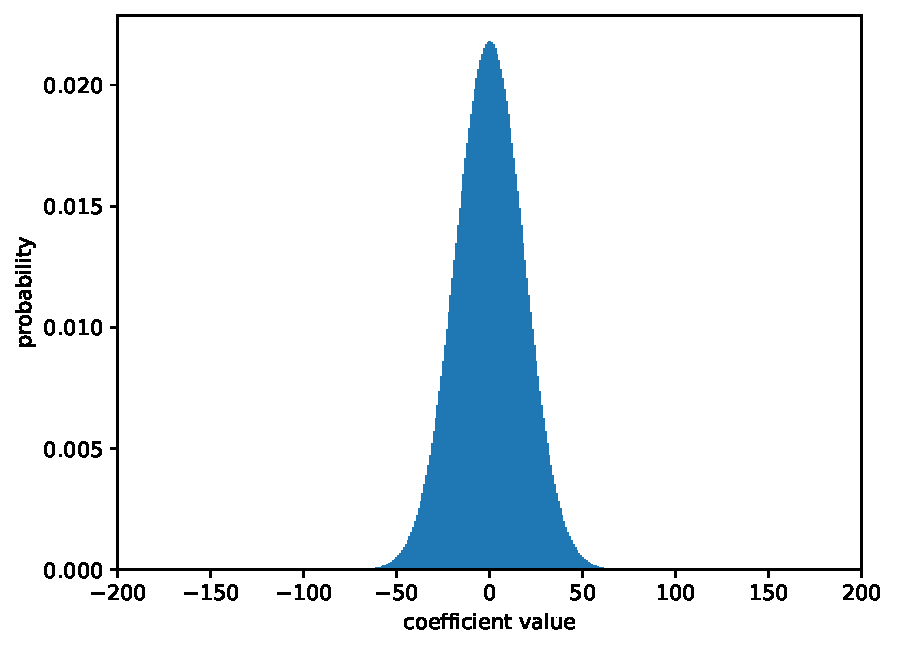
\includegraphics[width=.95\linewidth]{plots/dilithium_l3_cs_plot}%
		\caption{Dilithium (Security Level 3)}%
	\end{subfigure}%
	\begin{subfigure}{.5\textwidth}%
		\centering%
		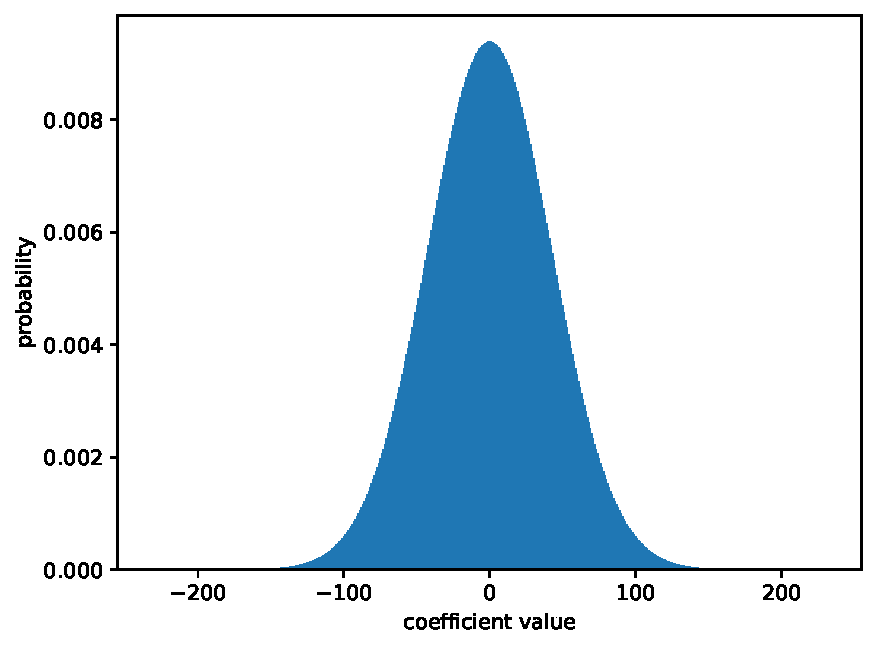
\includegraphics[width=.95\linewidth]{plots/qtesla_l3_cs_plot}%
		\caption{qTESLA (Security Level 1)}%
	\end{subfigure}\\\vspace{1em}%
	\begin{subfigure}{.5\textwidth}%
		\centering%
		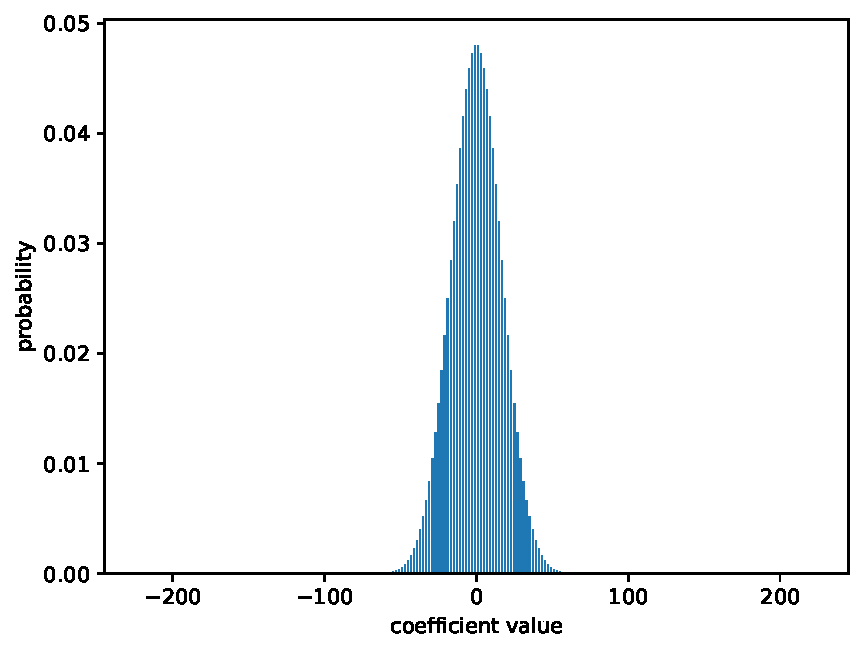
\includegraphics[width=.95\linewidth]{plots/bliss_l3_cs_plot}%
		\caption{BLISS (BLISS-III)}%
	\end{subfigure}%
%
	\caption{The distribution of a $cs$-coefficient (same as that of a faulted $z$-coefficient) for the different signature schemes. The plots for Dilithium and BLISS show the entire distributions. The plot for qTESLA shows the $6$-$σ$-interval of the $cs$ distribution.}
	\label{fig:csdist}
\end{figure}


The heavy lifting of classifying whether a coefficient of $y$ is zero or not is done by the ILP-solver.
Nevertheless for a certain set of equations we can say with ease that the corresponding $y$-coefficient can not be zero.
When a coefficient $y_{i}$ is zero we know that $z_{i} = (c s + 0)_{i}$. For all signature schemes we can give a bound $b$ to the maximum possible absolute value a coefficient of $cs$. Thus if $\lvert z_{i} \rvert>  b$, we know that $y_{i} \neq 0$ with a probability of $1$.

For improved performance we will thus remove any equations where we can tell, by using the aforementioned approach, that their corresponding $y$-coefficient is not zero. We do this before passing these equations to the ILP-solver. In practice this means removing the corresponding entry in the vector $z'$ and the corresponding row in the matrix $C$.

To go even further we can use a lower threshold $t < b$ to pre-filter our equations. Because for all three  signature schemes we know that the distribution of $cs$ has most of its probability mass close to zero, is symmetrical and thus has very little probability mass near the bounds $-b$ and $b$, this will filter out even more equations which are not affected by a fault. On the contrary we will also filter out some equations which were indeed affected by the fault increasing the amount of signatures we need. For a better visualization of the distributions see Figure \ref{fig:csdist}
\todo{maybe compare plots ot cs+y with y!=0}

%. Thus choosing a threshold $t < b$ we will thus need more signatures to perform our attack.
%This tradeoff between the amount of signatures required and the false-positive rate of the linear equation set we will be passing to the ILP-solver will be evaluated for Dilithium in section \ref{sec:evalthreshold}.


The metric we control by pre-filtering the equations is
%With pre-filtering we are able to control
the false-positive rate of our equation set. Here we classify an equation as being true, i.e. $y_{i} = 0$ or not. A true-positive classification would be if we classify an equation is faulted and it indeed is. A false-positive classification is when we classify an equation as faulted, although it actually is not. Thus the false-positive rate is ratio of the number false-positive classifications of our equations to the total number of equations. This number is an interesting metric for the efficiency of our attack as we will discuss later.
We are able to control this number by two parameters:
\begin{enumerate}
	\item the iteration number $m$, after which we induce a fault.
	\item the cutoff value $t$ we use for filtering
\end{enumerate}







\section{Attacking Dilithium}
\label{sec:attackdilithium}

In this section we will discuss the Dilithium signature scheme specific details for our attack.

\subsection{Implementation assumptions and attacker model}
First we assume that a big loop with $nl$ iterations will sample the coefficients for all $l$ polynomials with $n$ coefficients each in $\bm{y}$. Secondly we assume that the shuffling occurs throughout all the polynomials of the vector $\bm{y}$. This means that coefficients which where faulted to be zero located in the last polynomial may be shuffled to another polynomial, e.g. the first one.

We thus adjust our attacker model in the way that the attacker will induce a fault after the $1 \leq m \leq nl$ iteration in the loop which samples the coefficients of the masking polynomials.

\subsection{One ILP per polynomial}
The Dilithium signature scheme calculates the signature like follows:
\begin{align}
	\bm{z} = \bm{s}_{1} c + \bm{y}
\end{align}
Where $\bm{z}, \bm{s}_{1}, \bm{y} \in \mathcal{R}_q^{l}$ and $c \in \mathcal{R}_q$. We thus can not directly apply the attack mentioned before.
To still use our attack against Dilithium, let $\bm{z}_{i}, {\bm{s}_{1}}_{i}, \bm{y}_{i}$ be the $i$'th polynomial in the respective vectors for $1 \leq i \leq l$.
According to definition of $\bm{z}$ it holds for all $1 \leq i \leq l$ that $\bm{z}_{i} = c {\bm{s}_{1}}_{i} + \bm{y}_{i}$. Now, because $\bm{z}_{i}, c, {\bm{s}_{1}}_{i}, \bm{y}_{i} \in \mathcal{R}_q$ we can apply our attack for every $i$ to recover once secret polynomial of $\bm{s}_{1}$ at a time, eventually recovering the entire vector $\bm{s}_{1}$.

\subsection{Bound for the difference $z_{i}' - C_{i}s'$ and threshold $t$}
The coefficients of the commitment polynomial $c$ have at most an absolute value of $1$ which can occur at most $\tau$ times. The coefficients of the $\bm{s}_{1}$ polynomials have at most an absolute value of $\eta$. Thus we know that $\lvert  C_{i}s' \rvert \leq \tau \eta = \beta$. Finally the coefficients of the $\bm{y}$ masking polynomials have an absolute value of at most $\gamma_{1}$, thus $\lvert z'_{i} \rvert$ is at most $\tau \eta + \gamma_{1} = \beta + \gamma_{1}$. The absolute value of the difference is consequently $K = 2 \beta + \gamma_{1}$.

To filter equations we will use a threshold of $t = \beta$ as this is the upper bound for coefficients in $\bm{s}_{1}c$.% as we just discussed in the previous sections.

\subsection{Creating signatures using only \texorpdfstring{$\bm{s}_{1}$}{\textbf{s}1}}
In the Dilithium signature scheme $\bm{s}_{1}$ is only one part of the secret key. Our attack can not recover the second part of the secret key, $\bm{s}_2$, still $\bm{s}_{1}$ is enough information for an attacker to sign arbitrary messages. To sign arbitrary messages two different methods were previously presented. One by Bruinderink and Pessel \cite[pp.~33--34]{Groot_Bruinderink_Pessl_2018} and one by Ravi et al. \cite[pp.~12--13]{ravi_2018}. These signatures are indistinguishable from real ones when only given the public key. Only given the secret key we can distinguish the signatures created using only $\bm{s}_{1}$ from the ones created by someone with the entire secret key. 


\section{Attacking qTESLA}
\label{sec:attackqtesla}
Attacking qTESLA is straight forward because the qTESLA signature scheme strictly follows our general attack approach we presented in section \ref{sec:attackfinally}. Thus we only have to consider the maximum difference $z'_{i} - C_{i}s'$ and the appropriate threshold $t$.

\subsection{Bound for the difference $z_{i}' - C_{i}s'$ and threshold $t$}
\label{sec:qteslathreshold}
The polynomial $s$ has coefficients which follow the discrete gaussian distribution with standard deviation $\sigma$. This distribution is a long-tailed one and it can have theoretically infinitely large samples (coefficients). In practice discrete gaussian samplers have a parameter $\tau$ which defines a so called cutoff-value $\tau \sigma$, which limits the samples to be in the domain $[-\tau \sigma, \tau \sigma] \cap \mathds{Z}$. For our evaluation we choose $\tau = 6$ because this is the default one used in SageMath \cite{WEB:Sage}. Thus we can limit the domain of $s$ to be $[-\tau \sigma, \tau \sigma] \cap \mathds{Z}$.% This estimation is very conservative and better results may be possible by choosing a smaller $\tau$ when computing the threshold $t$.

The commitment value $c$ has exactly $h$ non-zero coefficients which are $-1$ or $1$ and the rest is zero. Thus we know that the polynomial $cs$ has coefficients in the range $[-h \tau \sigma, h \tau \sigma] \cap \mathds{Z}$.

The masking polynomial $y$ has per definition coefficients in the range $[-B, B] \cap \mathds{Z}$. Thus we can say that the coefficients of $z = y+cs$ are in the interval $[-B h \tau \sigma, B h \tau \sigma] \cap \mathds{Z}$.
Now looking at the difference $z'_{i} - C_{i}s'$ we know that that it's maximum absolute value is bounded by $2 h \tau \sigma + B$. Thus we choose $K = 2 h \tau \sigma + B$ and $t = h \tau \sigma$.


\section{Attacking BLISS}
\label{sec:attackbliss}
The BLISS \cite{bliss} signature scheme was first introduced by Léo Ducas et al. in 2013. With their novel rejection sampling algorithm and other modifications they were able to significantly reduce the standard deviation of their signatures and thus the signature size compared to other post-quantum secure schemes at that time. Their new rejection sampling algorithm is based on the bimodal gaussian distribution. This distribution is obtained in their scheme by choosing a random bit $b \in \{0, 1\}$ and computing a signature vector $z_{1} = y_{1} + (-1)^{b} s_{1}c$. The entire signature algorithm can be found in section \ref{sec:blissdesc}.


%\subsection{Special considerations}
Note that the previous two signature schemes do not use such a bit in their signature generation algorithms. To adapt our attack to BLISS we will have to include this bit of information in the ILP.
%For a single signature this is just a single bit of information, but as we require more signatures because we fault after more iterations the entropy will grow exponentially and the bits will be harder to recover.
%Despite this fact we were able to achieve good results for some of the proposed parameter sets of BLISS.
\todo{maybe add the out-commented paragraph to bliss results?}

\subsection{A modified ILP for BLISS}
Due to the random bit we now have three types of unknowns: The coefficients of the secret key polynomial $s_{1}$, the coefficients of the masking polynomial $y_{1}$ and the bit $b$.
Thus the ILP will use three classes of variables: In addition to $x$ and $\hat{s}$ we already described in the general ILP, we will have the binary variables $b_1, \ldots, b_σ \in \{0, 1\}$ to represent the random bit $b$.  

%Let $\hat{s} \in \{-2, -1, 0, 1, 2\}^{n}$ be the coefficient vector of $s_{1}$, let $x \in \{0, 1\}^{\sigma n}$ the binary / boolean vector which classifies whether a coefficient of one of the $y_{1}$'s is faulted or not just like we described in detail in section \ref{sec:ilpvars}. Finally let $b_{1},  b_{2}, \ldots, b_{\sigma} \in \{-1, 1\}^{\sigma}$ be the variables which describe the sign, which was induced by the bit $b$ ($(-1)^{b}$) for each signature .
%Here $\sigma$ denotes the amount of signatures we have acquired and $n=512$ for all BLISS parameter sets proposed by the authors.

Next will will define for all $1 \leq i \leq σ$ the vector $\vec{b}_i \in \{-1, 1\}^{n}$ as follows:%\footnote{Such a vector can not be straight forward be defined by a linear constraint, but with a small trick it is possible to construct something similar using a matrix vector product where the vector has $\sigma$ $\{0, 1\}$ entries which encode the signs.} \todo{probably explain the footnote in detail}
\begin{align}
	\vec{b}_i = (\overbrace{2(1-b_{i})-1, 2(1-b_{i})-1, \ldots, 2(1-b_{i})-1}^{n \text{ times}})^t\end{align}

This allows us to create the vector $\dot{b}$ which we define as all $\vec{b}_i$ vectors vertically stacked on one another, just like the definition of e.g.  $\dot{z}$.

Finally we can redefine the two constraints \eqref{constraint_leq} and \eqref{constraint_geq} of the ILP as follows,% Do note that additional constraints do define the domain of the different variables are required.
\begin{align}
	\label{constraint_leq_bliss}
	\dot{z} - \dot{b} \cdot C\hat{s} & \leq K (1 - x) \\
	\label{constraint_geq_bliss}
	\dot{z} - \dot{b} \cdot C\hat{s}  & \geq - K (1 - x)
\end{align}
where the $\cdot$ (dot) between $\dot{b}$ and $C\hat{s}$ denotes the entry-wise multiplication of the two vectors.


\subsection{Bound for the difference $z_{i}' - C_{i}s'$ and threshold $t$}
Let $d_{1} = \lfloor nδ_{1} \rfloor$ be the amount of $\pm1$ coefficients and $d_{2} =  \lfloor nδ_{2} \rfloor$ the amount of $\pm2$ coefficients in $s_1$.
Note that $c$ has exactly $κ$ coefficients with at most an absolute value of $1$ and the rest zero. Thus we maximize $C_i s'$ if all  $\pm2$-coefficient of $s_1$ match with non-zero coefficients of $C_i$ and the remaining $κ - d_2$ non-zero coefficients of $C_i$ match with the $\pm1$-coefficients in $s_1$. As for all parameter sets $κ > d_2$ holds, the bound for the absolute value of $C_i s'$ is  $2 d_{2} + κ - d_{2} = d_2 + k$,
%For all by the authors proposed parameter sets $C_{i}s'$ has at most an absolute value of $2 d_{2} + κ - d_{2} = d_2 + k$. \todo{why is that so, explain the calculation}
which we will use as the threshold.

The coefficients of $y_{1}$ follow the discrete gaussian distribution with a standard deviation $σ$. As already discussed in detail in section \ref{sec:qteslathreshold} we can limit the absolute values of the coefficients of $y_{1}$ to $τ σ$ with $τ = 6$. Thus we know that $\lvert z_{i}' \rvert \leq d_{2} + κ + τ σ$. Thus we choose $K = 2 (d_{2} + κ) + τ σ$.


\subsection{Recovering the entire secret key}
This attack will only recover the secret polynomial $s_{1}$ but not the second secret polynomial $s_{2}$. This is not a problem as $s_{1}$ is sufficient to recover the entire secret key: $s_2 = a_1 s_1 / 2 \bmod q$. This holds because:
\begin{align}
	a_{1}s_{1} / 2 = ((2g+1) / f)  s_{1} =  ((2g+1) / f)  f = (2g+1) f/f = 2g+1 = s_{2} \mod{q}
\end{align}







% !TEX root = ../my-thesis.tex
%




\chapter{Attack evaluation}
In this chapter we will quantify the effectiveness of our attack. We will begin by explaining our assumptions and evaluation strategy in section \ref{sec:attackeval:prelim}. In section \ref{sec:simresults} we will then present our results for Dilithium, qTESLA and BLISS respectively.  

\section{Preliminaries}
\label{sec:attackeval:prelim}
In this section we will discuss on what assumptions we base our simulations and what kind of parameters we will evaluate. 
\subsection{Assumptions}
\label{sec:simassumptions}
We assume an attacker as described in section \ref{sec:attackmodelgeneral}.
Further will always assume that we as the attacker will have at least as much information as would be sufficient to break the signature scheme if the shuffling countermeasure would not be used. This translates to the fact that we will always have $n$ or more faulted coefficients which correspond to at least $n$ linear independent equations. This is because without the shuffling countermeasure an attacker would know which coefficients were faulted (the last few), take the corresponding linear equations and solve them using gaussian elimination.



\subsection{Notion of success}
\label{sec:simsuccess}
For a certain $m$ we will say that we were successful in breaking the signature scheme, if we manage to succeed recovering the entire secret in at least two out of three tries, i.e. we have a success rate of at least around $66\%$. Each try fails after a timeout of 5 minutes wall time.

\subsection{Parameter evaluation}
When we use only the minimal mount of signatures required to fulfill our aforementioned requirements the attack will not show optimal results.
Thus, for Dilithium, we will evaluate two parameters of our attack which we hope to improve our results:
\begin{enumerate}
	\item surplus of equations $p$
	\item threshold $t$
\end{enumerate}
For qTESLA and BLISS we will only evaluate the parameter $p$. 

The surplus of equations $p$ is the minimal amount of additional faulted equations, relative to the minimum described in  \ref{sec:simsuccess}.
In our simulations we control this value by generating signatures until we can guarantee that we have has at least $n + p$ faulted equations out of which where exist $n$ linear independent ones. Note that using this approach the resulting amount of faulted equations may be higher than the surplus of equations parameter, because a single signature might produce more than one faulted signature.

The threshold parameter is used as to steer the false-positive rate as described in detail in section \ref{sec:prefilter}. The lower the threshold, the lower the false-positive rate and vice versa.
The false-positive rate is dependent on both, $m$ and $t$. Thus for a fixed $m$ the false-positive rate only depends on $t$.

We choose the two parameters based on the following two arguments:

We argue that a greater surplus of equations opens more choices to the ILP-solver to classify enough equations properly and thus the searchspace will more likely contain an easy-to-find path to a solution.
The arguing with the false-positive rate is that a lower false-positive rate makes (random) positive classification guesses of the ILP-solver more likely to be correct and thus the ILP-solver should reach its objective quicker, eventually recovering the secret polynomial. Additionally a lower false-positive rate reduces the total amount of equations required to have at least $n$ true equations. This reduces the amount of total variables and thus the difficulty of the generated ILP instance.


We tested our hypothesis statistically by running attack simulations for Dilithium (NIST security level II) for $f = 1, \ldots 10$. Recall that $f$ denotes the amount of faulted coefficients. We do not choose higher $f$ because we empirically know our attack almost always succeeds in that case.



\begin{figure}%
		\centering%
		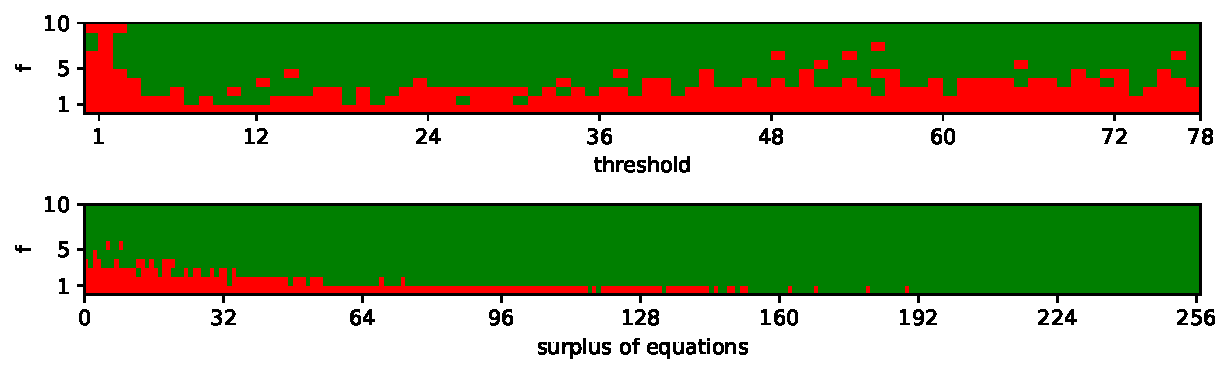
\includegraphics[width=.95\linewidth]{plots/threshold_pccolormesh}%
		%\caption{threshold ($s$)}%
	\caption{Heatmap showing the correlation between threshold and success as well as the correlation between surplus and success for $f = 1, \ldots,10$. A red rectangle indicated a failed attack, a green rectangle indicated a successful attack.}
	\label{fig:heatmap}%
\end{figure}

The heatmap \ref{fig:heatmap} clearly shows that the surplus parameter has an effect on the attack performance which is also confirmed by the Pearson correlation coefficients in Figure \ref{fig:corrs}.
For the threshold parameter on the other hand this is not directly clear. Our data shows that the attack performance is poor when extremely low thresholds are used. We think that an extremely low threshold affects a parameter other than the false-positive rate and this to us unknown parameter has a negative impact on the attack performance.
This phenomena can also be seen in Figure \ref{fig:corrthreshold}: For $f \geq 6$, we see a positive correlation is caused by the poor attack performance with for extremely low thresholds. For smaller $f$ we see a negative correlation, due to the low  false-positive rate. While the absolute value of the correlation coefficient for $f \leq 5$  is not very big, taking into consideration that it also has to compensate for the poor performance when the threshold is extremely low, the positive effect of the threshold to the attack performance is not neglectable.

\begin{figure}%
	\centering%
	\begin{subfigure}{.5\textwidth}%
		\centering%
		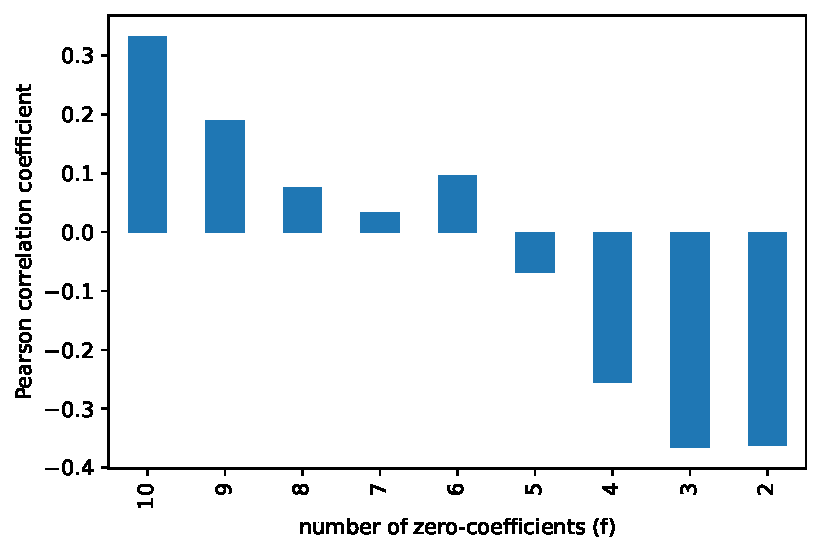
\includegraphics[width=.95\linewidth]{plots/threshold_correlation}%
		\caption{threshold $t$}%
		\label{fig:corrthreshold}%
	\end{subfigure}%
	\begin{subfigure}{.5\textwidth}%
		\centering%
		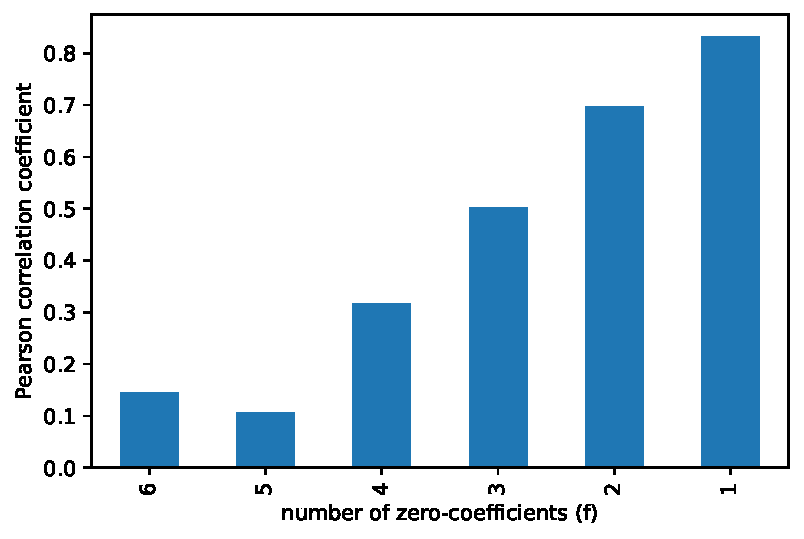
\includegraphics[width=.95\linewidth]{plots/surplus_correlation}%
		\caption{surplus of equations $s$.}%
		\label{fig:corrsurplus}%
	\end{subfigure}%
%
	\caption{The minimal required surplus of equations and the corresponding signature count per $f$. If a bar is not present it means that no surplus was required for that security level and $f$.}
	\label{fig:corrs}%
\end{figure}




When we perform an attack with default parameters, we mean we will use a threshold which does not filter any true-positive equations, we fulfill the assumptions defined in section \ref{sec:simsuccess} and all that with the minimal amount of signatures required.



\subsection{Parameter evaluation strategy}
In general the simulations aim to find out how lax we can be in the timing of the fault, which translate to how high we can go with the iteration number $m$, after which we will induce a fault. While in the simulations we will fault exactly $f$ coefficients per signature, the simlation results can be translated to an attacker who faults on average $f$ coefficients per signature.




    \begin{algorithm}
        \SetKwFunction{print}{print}
        $t \gets \beta$ \tcp{threshold}
        $f \gets nl$ \tcp{number of zero-coefficients; $m = nl - f$}
        \While{$f \geq 1$ and $t \geq 1$}{
            \eIf{at least $2$ out of $3$ attacks successful}{
                \print{for $f$ zero-coefficients we need a threshold of no more than $t$}\;
                $f \gets f - 1$\;
            }{
                $t \gets t - 1$\;
            }
        }
        
        \caption{Evaluation strategy for the $s$ parameter.}
        \label{alg:surplus}
    \end{algorithm}
    
    %\phantom{hi}
    \vspace{4em}
    
    \begin{algorithm}
        \SetKwFunction{print}{print}
        $s \gets n$ \tcp{surplus}
        $f \gets nl$ \tcp{number of zero-coefficients; $m = nl - f$}
        \While{$f \leq 1$ and $s \leq 2n$}{
            \eIf{at least $2$ out of $3$ attacks successful}{
                \print{for $f$ zero-coefficients we need a surplus of at least $s$}\;
                $f \gets f - 1$\;
            }{
                $s \gets s + 1$\;
            }
        }
        
        \caption{Evaluation strategy for the $t$ parameter.}
        \label{alg:threshold}
    \end{algorithm}






%The parameters $p$ % and $t$
%will be evaluated as follows: We start with $m_0 = s_0 = 0$ and as long as our attack succeeds we increment $m$ by one and continue our simulations. When we reach a $m$ where we do not succeed with our current $s$ we will repeat the simulation for the same $m$ but an incremented $s'$, which is calculated as the previous amount of faulted equations incremented by $1$. Note that the previous amount of faulted equations may be higher than $s$, as $s$ is defined a minimum. When we reach a $s$ where our attack succeeds we again continue to only incrementing $m$ until again our attack does not succeed anymore and we repeat the strategy.

%When evaluating the parameter $t$ we will start with $m = 0$ and a $t$ which does not filter any true-positive equations. We increment $m$ until our the attack fails. If that is the case we decrement $t$ by one and try again for that $m$ until we succeed. Once we reached a $t$ where we succeed we again begin to increment only $m$ until again our attack does not succeed anymore and we repeat the strategy.

The evaluation strategy for the parameter \say{surplus of equations} and \say{threshold} are depicted in Algorithm \ref{alg:surplus} and \ref{alg:threshold} respectively.
Using these strategies we will be able to determine for every $m$ if our attack succeeds, and if yes, what parameter value is necessary for success.

\subsection{Simulation hard- and software}
\label{sec:practise_server}
The ILP-solver used for our simulations is Gurobi \footnote{\url{https://www.gurobi.com/}}.
Our simulation is written in Python using the Numpy library \footnote{\url{https://numpy.org/}} and the gurobipy library \footnote{\url{https://pypi.org/project/gurobipy/}} for the Gurobi Python bindings. All simulations were run on a computer with a Intel\textsuperscript{\textregistered} Xeon\textsuperscript{\textregistered} Processor E7-4870 (4 sockets, 10 cores, using 40 out of 80 available threads @ 2.4GHz) with 500GB of RAM.


\section{Simulation results}
\label{sec:simresults}
In this section we will discuss the results of our simulations. First we will start with a thorough discussion on the results for Dilithium, as we will evaluate and compare both the parameters $s$ and $p$. Next we will follow with qTESLA as well as BLISS. In the end we will discuss how the repetition rate affects the required amount of signatures.

\subsection{Dilithium}
For Dilithium we will first discuss the results when our default parameters are used. Then we will discuss the results for both, the parameter $s$ and the parameter $t$. Finally we will compare the results of both parameters.

\subsubsection{Default parameters}
\label{sec:min_sig_amount}

\begin{figure}
	\centering
	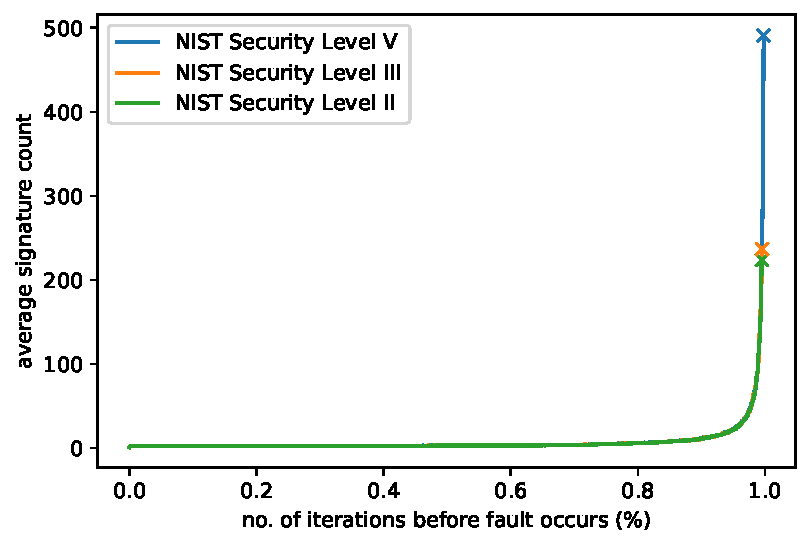
\includegraphics[width=.7\linewidth]{plots/dilithium_sigcount_noparams}
	\caption{Average amount of signature required for a successful attack per $m$ in percent (relative to $nl$). The amount of signatures is very similar throughout all security levels for early iteration aborts. Thus the green line covers the other two. Crosses indicate the maximum signature count.}
	\label{fig:dilithiumsigcountnoparams}
\end{figure} 

When using the default threshold described in section \ref{sec:prefilter} and a surplus of $0$ our attack succeeds for $f$ as low as $5$, $6$ and $4$ requiring $224$, $236.5$ and $491$ signatures on average for the NIST security levels II, III and V respectively.
Further we observe that the higher the NIST security level the more signatures are required. This is due to the fact that minimum amount of equations increases as the security level increases  because the parameter $l$ increases for every security level.  Recall that the minimum amount of required equations is $nl$ for Dilithium. The amount of signatures required per $m$ is depicted in Figure \ref{fig:dilithiumsigcountnoparams}.

\subsubsection{Surplus of equations}
\label{sec:dilithiumsurplus}

\begin{figure}%
	\centering%
	\begin{subfigure}{.5\textwidth}%
		\centering%
		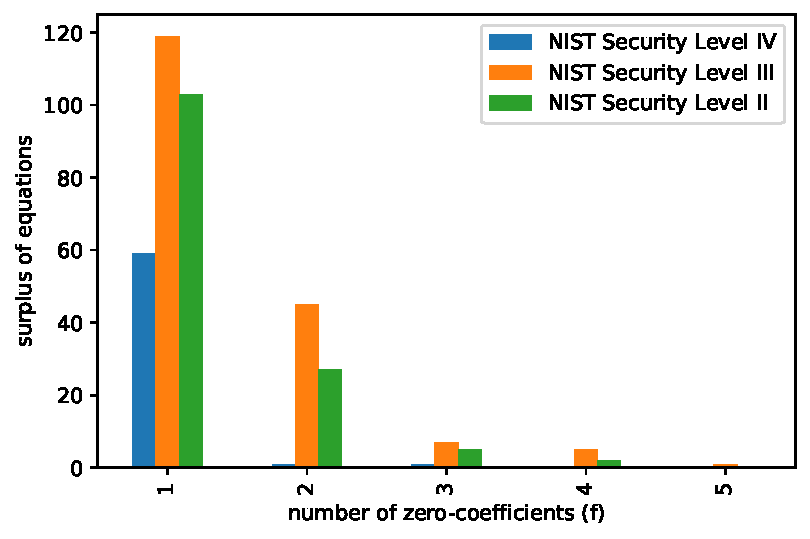
\includegraphics[width=.95\linewidth]{plots/dilithium_surplus}%
		\caption{Surplus of equations per $f$}%
		\label{fig:dilithiumsurplus}%
	\end{subfigure}%
	\begin{subfigure}{.5\textwidth}%
		\centering%
		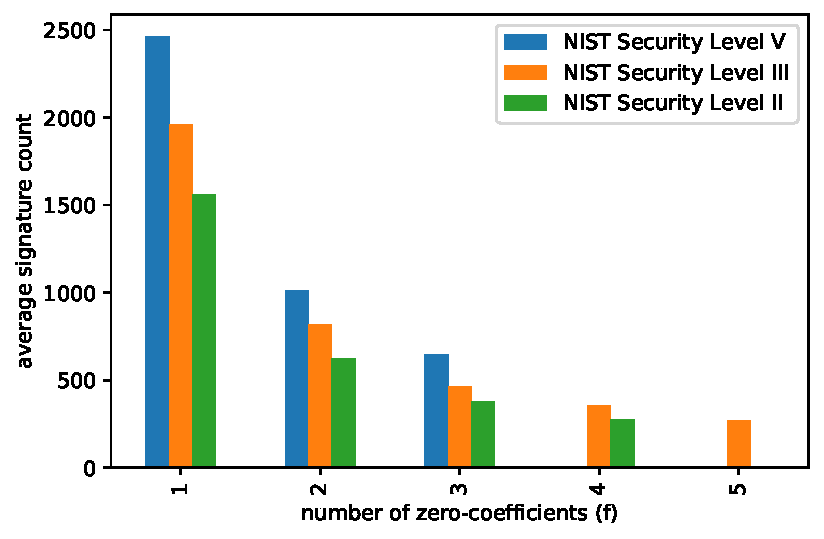
\includegraphics[width=.95\linewidth]{plots/dilithium_sigcount_upper}%
		\caption{Corresponding signature count per $f$.}%
		\label{fig:dilithiumsigcountsurplus}%
	\end{subfigure}%
%
	\caption{The minimal required surplus of equations and the corresponding signature count per $f$. If a bar is not present it means that no surplus was required for that security level and $f$.}
	\label{fig:dilithiumsigcountsurplussurplus}%
\end{figure}

Our simulation results show, that for every $m$, we are able to succeed our attack.
This means that an attacker who is able to (on average) fault a single coefficient of $\bm{y}$ can recover $\bm{s}_{1}$, given that he can do it on around $1562$,  $1959.5$, $2465$ signatures for NIST security level II, III and V respectively. The surplus of equations required per $m$ as well as the amount of signatures required per $m$ are depicted in Figure \ref{fig:dilithiumsigcountsurplussurplus}.

We can observe that the signature count increases as $f$ decreases, as well as when the security level increases. First is due to the fact that we get less zero-coefficients per signature and letter is the case because higher security levels require more zero-coefficients in total ($nl$ many) as $l$ increases as the security level does.



\subsubsection{Threshold}
\label{sec:evalthreshold}

\begin{figure}%
	\centering%
	\begin{subfigure}{.5\textwidth}%
		\centering%
		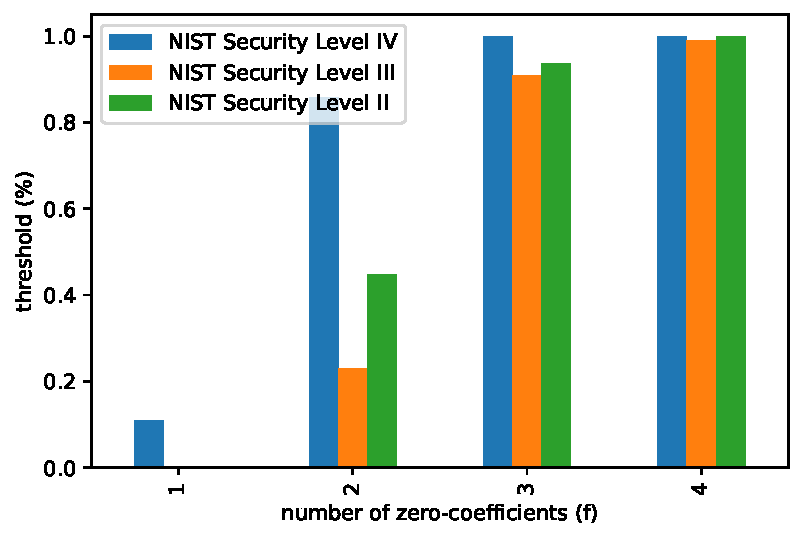
\includegraphics[width=.95\linewidth]{plots/dilithium_threshold_percent}%
		\caption{Maximum possible threshold ($\%$).}%
		\label{fig:dilithiumthreshold}%
	\end{subfigure}%
	\begin{subfigure}{.5\textwidth}%
		\centering%
		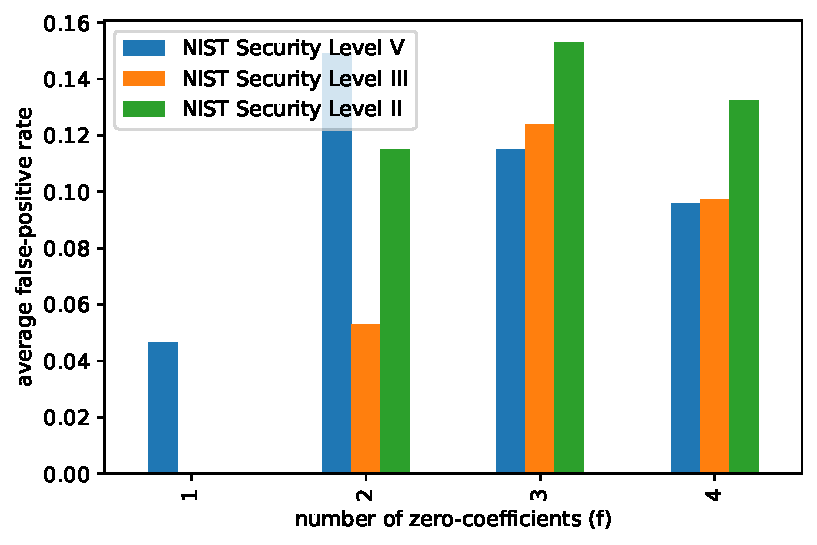
\includegraphics[width=.95\linewidth]{plots/dilithium_threshold_fpr}%
		\caption{Corresponding false-positive rate.\phantom{}}%
		\label{fig:dilithiumthresholdfpr}%
	\end{subfigure}\\\vspace{1em}%
	\begin{subfigure}{.5\textwidth}%
		\centering%
		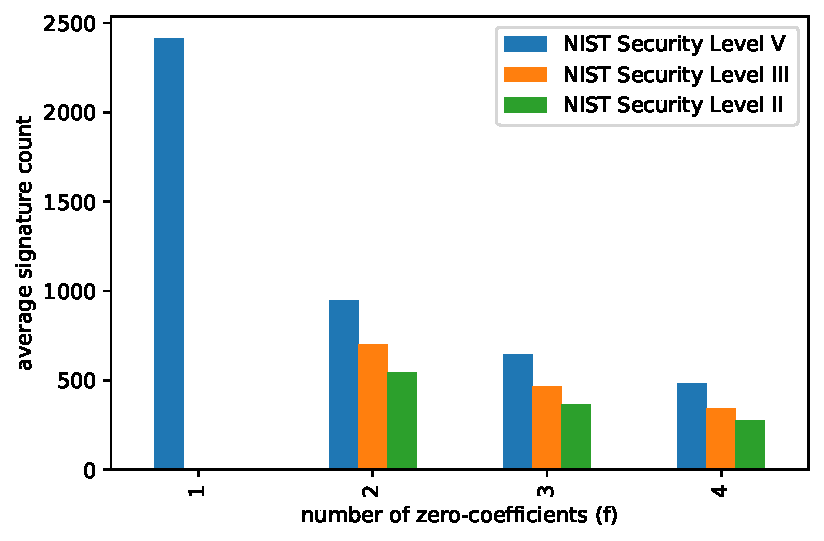
\includegraphics[width=.95\linewidth]{plots/dilithium_threshold_sigcount}%
		\caption{Corresponding signature count.}%
		\label{fig:dilithiumthresholdsigcount}%
	\end{subfigure}%
%
	\caption{The maximum possible threshold per $f$ and the corresponding false-positive rate as well as the corresponding signature count.}
	\label{fig:dilithiumthresholdall}%
\end{figure}
We evaluated the threshold parameter for $f \leq 4$ as for higher $f$ our attack succeeded without needing a reduced threshold.
We were able to succeed our attack for all $f \geq 2$ for all NIST security levels. With a single coefficient faulted our attack succeeded only for security level V.

In Figure \ref{fig:dilithiumthreshold} we observe that as $f$ decreases ($m$ increases) we require a lower threshold to succeed. This can be explained because as $f$ decreases for a fixed threshold we will have an increased false-positive rate. To achieve the same or lower false-positive rate as we had with $f + 1$ we require a lower threshold. 

Comparing the threshold of different security levels for a fixed $f$ is difficult because the distributions of $c\bm{s}_1$ differs for different the security levels. This kind comparison is better performed by looking at the false positive rate. 

%If we compare the relative threshold for fixed $f$ but different security levels we notice that the relative thresholds are similar for $f = 3, 4$, but very different for $f = 1$. Latter we can not properly explain. It might be due to lucky/unlucky ILP instances.

Inspecting the false-positive rate in Figure \ref{fig:dilithiumthresholdfpr} for $f=3, 4$ we observe that the higher the security level the lower the false-positive rate. This behavior is expected as $l$ ILPs need to be solved per attack and $l$ increases as the security level increases. As all security levels have the same time limitation, higher security levels need to solve more ILPs per fixed time and thus have less time per ILP. To solve an ILP in a shorter timeframe the attacker requires easier ILP instances. Thus a lower false-positive rate is required. %Finally again we can not properly explain the data for $f=1$.

For $f = 2$ and security level V we are unable to properly explain the suddenly increasing false-positive rate. It might be that by chance, despite the high false-positive rate, the ILP instances were easy.

The signature count (Figure \ref{fig:dilithiumthresholdsigcount}) increases as $f$ decreases and also for a fixed $f$ the signature count increases as the security level does.
Both of these phenomena have been explain in the previous section \ref{sec:dilithiumsurplus}.

\subsubsection{Comparison}
\label{sec:dilithiumcompare}
Looking at the aspect of for which $f$ we are able to perform a successful attack we can see that when using the \say{surplus of equations} parameter we can do so for any $f$ and any security level, whereas using the \say{threshold} parameter we are only able to do so for for all $f \geq 2$ and $f = 1$ only for security level V. 
The amount of signatures required is similar for both parameters.
%When comparing the amount of signatures which are needed for a successful attack per $f$ we  observe that when using the \say{surplus of equations} parameter we need slightly more signatures to succeed than with \say{threshold}.

%We value the fact that we are able to succeed with a higher $m$ more than the slightly decreased signature amount.
Thus we conclude that the parameter \say{surplus of equations} has a bigger impact on the attack performance than \say{threshold}.
Albeit we note that both parameters have impact on the attack performance. While the optimal solution is probably to use both parameters together with a certain weight, the attack results of the \say{surplus of equations} parameter are good enough for our use-case so that we will not do further research to increase the performance.
Additionally, because the attack strategy is very similar for the other two signature schemes, we believe that the results we obtained for Dilithium can also be applied to the other two signature schemes. Thus we will only evaluate the \say{notion of success} parameter for qTESLA and BLISS.

\subsection{qTESLA}

\begin{figure}[p]
\centering
\begin{subfigure}{.5\textwidth}
  \centering
  
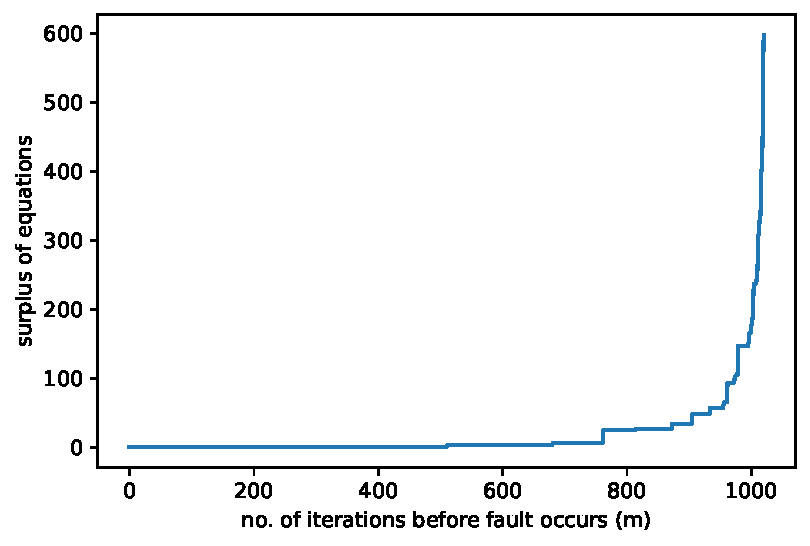
\includegraphics[width=.9\linewidth]{plots/server_qtesla_i_surplus}%
  \caption{Surplus of equations per $m$.}
  \label{fig:resqteslasurplus}
\end{subfigure}%
\begin{subfigure}{.5\textwidth}
  \centering
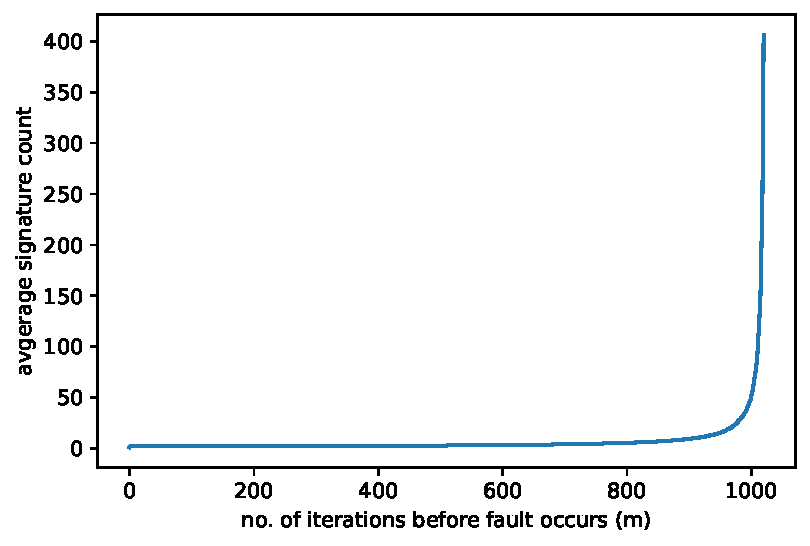
\includegraphics[width=.9\linewidth]{plots/server_qtesla_i_sigcount_surplus}%
  \caption{Corresponding signature count per $m$.}
  \label{fig:resqteslasigs}
\end{subfigure}

\caption{qTESLA (NIST security level I) simulation results. The minimal required surplus of equations and the corresponding signature count per $m$.}
\label{fig:resqtesla}
\end{figure}



%When evaluating the parameter we choose to increase it by 10 whenever the attack fails. We do this because in depending on the parameter set qTESLA's $n$ is 4 or 8 times as large as in Dilithium's and thus the increase of the parameter relative to $n$ is smaller. To finish our simulations in a reasonable amount of time we therefore increase the step size.

Our simulation results show that we are able to break the shuffling countermeasure for the parameter set \texttt{qTESLA-p-I} (NIST security level I) but not so for the parameter set  \texttt{qTESLA-p-III}  (NIST security level III) for any reasonable $m$.
When attacking security level I using the default parameters our attack succeeds for all $m \leq 510$. Using the \say{surplus if equations} parameter we were able to succeed with only two faulted coefficients for which we require on average of $406$ signatures. The exact results for security level I can be found in Figure \ref{fig:resqtesla}.
 
Compared to Dilithium and BLISS qTesla works on a way higher dimension even in the NIST security level I ($n = 1024$). Thus we assume this is the reason we were unable to break NIST security level III of qTESLA, as it doubles the dimension compared to security level I to $n = 2048$. Higher dimensions result in higher variable-count in the corresponding ILP, exponentially increasing the difficulty to solve it.

\subsection{BLISS}

\begin{figure}%
	\centering%
	\begin{subfigure}{.5\textwidth}%
		\centering%
		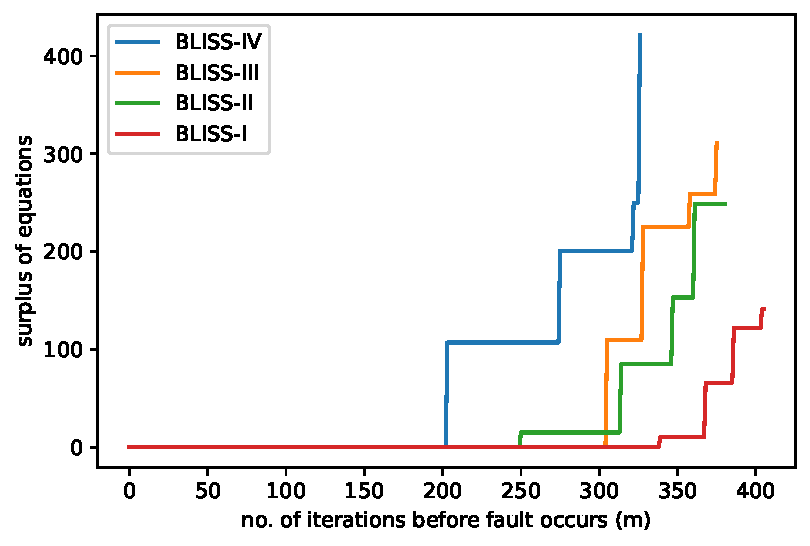
\includegraphics[width=.95\linewidth]{plots/bliss_surplus}%
		\caption{Surplus of equations per $m$.}%
		\label{fig:blisssurplus}%
	\end{subfigure}%
	\begin{subfigure}{.5\textwidth}%
		\centering%
		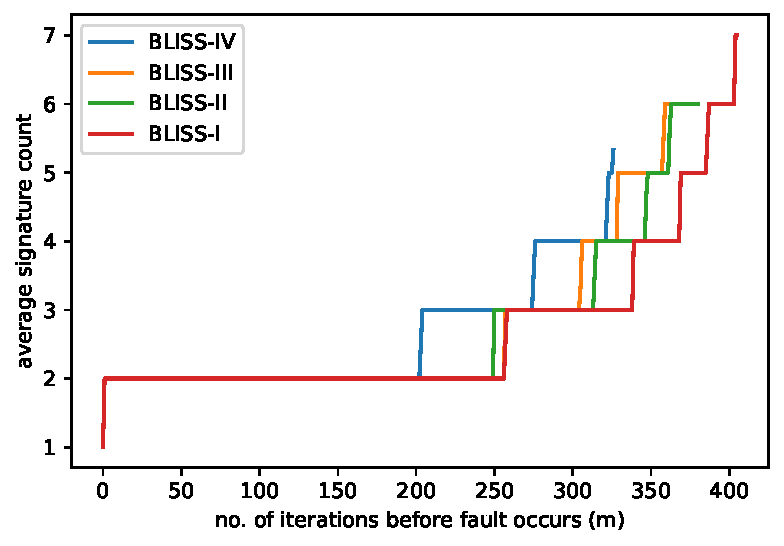
\includegraphics[width=.95\linewidth]{plots/bliss_surplus_sigcount}%
		\caption{Corresponding signature count per $m$.}%
		\label{fig:blisssurplussigcount}%
	\end{subfigure}%
%
	\caption{BLISS simulation results. The minimal required surplus of equations and the corresponding signature count per $m$.}
	\label{fig:blisssurplusandsigcount}%
\end{figure}


The authors of BLISS propose four different parameter sets, BLISS-I, BLISS-II, BLISS-III and BLISS-IV which aim to offer 128, 128, 160 and 192 bits of security respectively \cite[pp.~23--24]{bliss_full}. We were able to successfully attack all these parameter sets, though in contrast to Dilithium and qTESLA (NIST security level I) % and qTesla (\texttt{qTESLA-p-I})
we require the loop-abort to be more early. To be precise the loop-abort needs to occur at least prior the $405$th loop iteration, which is  around $80\%$ of the total iteration count.

The surplus of equations needed per $m$ and the corresponding required amount of signatures are depicted in Figure \ref{fig:blisssurplusandsigcount} for all BLISS parameter sets.



\subsection{Repetition rate and required amount of signatures}


All the schemes we attack are based on the Fiat-Shamir with aborts design. Thus these schemes may abort and retry. The expected amount of tries before the schemes output a valid signature is called the repetition rate. An attacker can not a priori know the repetition rate, thus he can not perfectly time his fault a priori. 

If the attacker model is strong enough such that an attacker can induce multiple loop abort faults during the signature generation, one for every possible repetition, the amount of signature required matches with the numbers we present here. If the attacker model is less strong, such that the fault can only be executed for one specific repetition count, e.g. only the first repetition, then the amount of signature required will increase, depending on the signature scheme and parameter set.

For deterministic signature schemes like Dilithium an attacker can generate a signature of a message $μ$ without fault and observe the repetition rate by time measurements. Using this repetition rate he can set a proper timing for the fault (loop abort in the last repetition) and sign $μ$ again, but this time with the a fault induced in the last repetition. Such an approach would double the amount of signature generations which need to be performed.

This does not work for probabilistic signature schemes, like BLISS and qTESLA. In this case an attacker has to set up the timing for a fault in the first repetition and repeat the signature generation until a signature is outputted after the first try. In this case the amount of signatures needed has to be scaled by the repetition rate of the particular scheme and parameter set.

qTESLA NIST security level I has an acceptance rate of $.13$ \cite[p.~452]{qtesla}, thus a repetition rate of  $7,69$. The amount of required signatures need to be scaled by $7,69$.
The repetition rates for Dilithium and BLISS can be found in Table \ref{table:dilithium} and \ref{table:bliss} respectively.

Finally we want to highlight that the repetition rate does not, other than the required signatures, affect our attack efficiency, e.g. difficulty of ILP instances or the false-positive rate. The repetitions performed for a particular signature can be detected by time measurements and thus signatures which did not match the expected repetition rate will be discarded and never appear in the actual attack data.



\begin{table}
\centering
\begin{tabular}{ c c c c }
 NIST Security Level & II & III & V \\ 
 \hline
 Repetition rate & $4.25$ & $5.1$ & $3.85$ \\  
\end{tabular}\vspace{1em}
\caption{Repetition rates for the Dilithium signature scheme \cite[p.~16]{dilithium_spec}.}
\label{table:dilithium}
\end{table}

\begin{table}
\centering
\begin{tabular}{ c c c c c }
 Parameter set & BLISS-I & BLISS-II & BLISS-III & BLISS-IV \\ 
 \hline
 Repetition rate & $1.6$ & $7.4$ & $2.8$ & $5.2$ \\  
\end{tabular}\vspace{1em}
\caption{Repetition rates for the BLISS signature scheme \cite[p.~24]{bliss_full}.}
\label{table:bliss}
\end{table}

% !TEX root = ../my-thesis.tex
%




\chapter{Conclusion, Countermeasures and future work}
Quantum computers may be able to break classic cryptography based on factoring and (elliptic curve) discrete logarithm soon. Thus we need post-quantum secure alternatives now. The NIST standardization process already revealed that Kyber is the recommended post-quantum secure key encapsulation mechanism and Dilithium the recommended post-quantum secure signature scheme to be standardized \cite{niststatus}.
Thus in the near future these schemes will be deployed on real devices, including  smartcards, microcontrollers and other devices susceptible to fault attacks but essential for our daily life. It is of great importance that before these devices are deployed in the real-world it is well known what attacks do exist and how to properly prevent them. While research on PQC fault attacks  has already been conducted \cite{espitau,Groot_Bruinderink_Pessl_2018,sensitivity,faultccm}%
%the effectiveness of the shuffling countermeasure has been overestimated.
, it was still far unclear whether the proposed countermeasures were sufficient.

In this thesis we showed how break one particular countermeasure, the shuffling countermeasure, which was so far assumed to be a sufficient countermeasure against loop-abort faults. 
%In this thesis we showed how to break this countermeasure.
We used multiple faulty signatures to construct a noisy equation system. We were able reduce the noise by filtering certain equations based on basic statistical analysis. Finally we constructed an ILP which was able to remove the last bit of noise and solve the equation system which revealed (part of) the secret key.
We demonstrated the attack effectiveness by attacking lattice-based signature schemes based of the Fiat-Shamir with aborts over rings type. We picked three signature schemes, namely the winner of NIST's PQC standardization process, Dilithium, as well as qTESLA and BLISS. Especially for Dilithium and qTesla's parameter set \texttt{qTESLA-p-I} we showed that the timing of the loop-abort is irrelevant, as long as at least one or two coefficients of the masking polynomial(s) are zero respectively. As such an event can occur with high probability under normal operation conditions for a single signature, it is hard to detect by software using the \say{check for zero} countermeasure. Our results highlight that more offensive research is needed on the proposed countermeasures and more additional countermeasures need to be proposed.
\section{Possible Countermeasures}
Bindel et al. \cite[p.~74]{sensitivity} presented a countermeasure against an attack, which skipped the addition of the entire masking polynomial $y$: Instead of adding the error polynomial on to the $sc$ vector, we add the $sc$ and $y$ into a new variable. This does not directly apply to our attack scenario as we do not cause $y$ to be zero by skipping its addition but instead we skip only part of its addition by skipping iterations in the sampling loop. Still, we can use this idea as a countermeasure against our attack by combining the sampling of $y$ and the addition of $y$ and $sc$ into a single loop, instead of doing both operations separately. Thus if we try to abort the loop which samples $y$, we also abort the addition of $sc$ and $y$. Consequently for all coefficients we fault, we only get uninitialized memory which does not contain any information. While this countermeasure is very efficient it only works for faults which target the execution flow of the program but it does not cover faults which for example target the programs memory.

As a possible countermeasure to protect BLISS, and possible other signature schemes which use the discrete gaussian distribution for their masking vectors, blinded gaussian shuffling can be used. This countermeasure was first introduced by Saarinen \cite[p.~82]{multishuffle} to counteract side-channel attacks against discrete gaussian sampler. The general idea is that then adding two discrete gaussian distributed random variables $X$ and $Y$ with a standard deviation of $\sigma$, centered at zero, $X + Y$ is also follows the discrete gaussian distribution, centered at zero with a standard deviation of $\sqrt{σ^{2} + σ^{2}}$. We can use this fact to construct a $y$-vector with standard deviation $σ$ by adding $k$ discrete gaussian distributed vectors with standard deviation $σ' = \frac{σ}{\sqrt{m}}$. Furthermore we shuffle all vectors before we add them together. This would require an attacker to perform $k$ loop-abort faults and still the expected amount of zero coefficients in the resulting masking vector would be exponentially small in $k$. Latter because a faulted-coefficient of a sampled polynomial might be added with a non-faulted coefficient the other vector due to the shuffling. Additionally this also protects against side-channel attacks. On the other hand this strategy also decreases the performance of the discrete gaussian sampler by $k$-fold. 


\section{Future work}
While we believe that our simulations already stress the need for more countermeasure research it would be interesting to see this attack to be implemented in practice on real hardware to further proof the point.
Additionally it might be possible to improve the performance of the attack by combining the $p$- and $t$-parameter in an optimal fashion. When evaluating \say{surplus of equations} parameter we choose a very conservative threshold.
Especially the qTESLA signature scheme was affected by the very conservative choice of the threshold, as this threshold was also used in the ILP as a constraint for the secret polynomial coefficient variables. A stricter constraint for these variables might improve the ILP performance and thus the attack performance.


%\part{Additional Example Part}
%% !TEX root = ../my-thesis.tex
%
\chapter{System}
\label{sec:system}

\cleanchapterquote{Innovation distinguishes between a leader and a follower.}{Steve Jobs}{(CEO Apple Inc.)}

\Blindtext[2][1]

\section{System Section 1}
\label{sec:system:sec1}

\Blindtext[1][2]

\begin{figure}[htb]
	
\includegraphics[width=\textwidth]{gfx/Clean-Thesis-Figure}
	\caption{Figure example: \textit{(a)} example part one, \textit{(c)} example part two; \textit{(c)} example part three}
	\label{fig:system:example1}
\end{figure}

\Blindtext[1][2]

\section{System Section 2}
\label{sec:system:sec2}

\Blindtext[1][2]

\begin{figure}[htb]
	
\includegraphics[width=\textwidth]{gfx/Clean-Thesis-Figure}
	\caption{Another Figure example: \textit{(a)} example part one, \textit{(c)} example part two; \textit{(c)} example part three}
	\label{fig:system:example2}
\end{figure}

\Blindtext[2][2]

\section{System Section 3}
\label{sec:system:sec3}

\Blindtext[4][2]

\section{Conclusion}
\label{sec:system:conclusion}

\Blindtext[2][1]
         % INCLUDE: system
%% !TEX root = ../my-thesis.tex
%
\chapter{Concepts: This text is here to test a very long title, to simulate the line break behavior, to show that an extremely long title also works}
\label{sec:concepts}

\cleanchapterquote{Users do not care about what is inside the box, as long as the box does what they need done.}{Jef Raskin}{about Human Computer Interfaces}

\Blindtext[2][1]

\section{Concepts Section 1}
\label{sec:concepts:sec1}

\Blindtext[2][2]

\section{Concepts Section 2 with a very very long title that illustrates how long section titles are handled in the footer}
\label{sec:concepts:sec2}

\Blindtext[3][2]

\section{Concepts Section 3}
\label{sec:concepts:sec3}

\Blindtext[4][2]

\section{Conclusion}
\label{sec:concepts:conclusion}

\Blindtext[2][1]
       % INCLUDE: concepts
%% !TEX root = ../my-thesis.tex
%
\chapter{Conclusion}
\label{sec:conclusion}

\Blindtext[2][1]

\section{System Section 1}
\label{sec:conclusion:sec1}

\Blindtext[2][2]

\section{System Section 2}
\label{sec:conclusion:sec2}

\Blindtext[3][2]

\section{Future Work}
\label{sec:conclusion:future}

\Blindtext[2][2]
     % INCLUDE: conclusion

% --------------------------
% Back matter
% --------------------------
%
{%
\setstretch{1.1}
\renewcommand{\bibfont}{\normalfont\small}
\setlength{\biblabelsep}{0pt}
\setlength{\bibitemsep}{0.5\baselineskip plus 0.5\baselineskip}
\printbibliography[nottype=online]
\newrefcontext[labelprefix={@}]
\printbibliography[heading=subbibliography,title={Webpages},type=online]
}
\cleardoublepage

%\listoffigures
%\cleardoublepage

%\listoftables
%\cleardoublepage

%\lstlistoflistings
%\cleardoublepage

%\appendix\cleardoublepage
%% !TEX root = ../my-thesis.tex
%
\chapter{Example Appendix}
\label{sec:appendix}

\Blindtext[1][1]

\section{Appendix Section 1}
\label{sec:appendix:sec1}

\Blindtext[1][1]

\begin{table}[h]
	\begin{tabularx}{\textwidth}{X | X | X}
		%\hline
		Alpha		& Beta			& Gamma			\\ \hline
		0			& 1				& 2				\\ \hline
		3			& 4				& 5				\\ %\hline
	\end{tabularx}
	\label{tab:table1}
	\caption{This is a caption text.}
\end{table}

\section{Appendix Section 2}
\label{sec:appendix:sec2}

\Blindtext[1][1]

\begin{table}[h]
	\begin{tabularx}{\textwidth}{X | X | X}
		%\hline
		Alpha		& Beta			& Gamma			\\ \hline
		0			& 1				& 2				\\ \hline
		3			& 4				& 5				\\ %\hline
	\end{tabularx}
	\label{tab:table2}
	\caption{This is a caption text.}
\end{table}

\Blindtext[1][2]
       % INCLUDE: appendix

%\cleardoublepage
%% !TEX root = ../my-thesis.tex
%
\pagestyle{empty}
\hfill
\vfill
\pdfbookmark[0]{Colophon}{Colophon}
\section*{Colophon}

This thesis was typeset with \LaTeXe.
It uses the \textit{Clean Thesis} style developed by Ricardo Langner.
The design of the \textit{Clean Thesis} style is inspired by user guide documents from Apple Inc.

Download the \textit{Clean Thesis} style at \url{http://cleanthesis.der-ric.de/}.


%\clearpage

\thispagestyle{empty}
\newpage
\thispagestyle{empty}
\mbox{}
\thispagestyle{empty}
\newpage
\thispagestyle{empty}
\mbox{}
\clearpage

% **************************************************
% End of Document CONTENT
% **************************************************
\end{document}
